\documentclass[10pt]{beamer}
\usetheme[
%%% option passed to the outer theme
%    progressstyle=fixedCircCnt,   % fixedCircCnt, movingCircCnt (moving is deault)
  ]{Feather}
  
% If you want to change the colors of the various elements in the theme, edit and uncomment the following lines

% Change the bar colors:
%\setbeamercolor{Feather}{fg=red!20,bg=red}

% Change the color of the structural elements:
%\setbeamercolor{structure}{fg=red}

% Change the frame title text color:
%\setbeamercolor{frametitle}{fg=blue}

% Change the normal text color background:
%\setbeamercolor{normal text}{fg=black,bg=gray!10}

\setbeamertemplate{caption}[numbered]
\setbeamertemplate{section in toc}[sections numbered]
\setbeamertemplate{subsection in toc}[square]
%\setbeamertemplate{bibliography item}{\insertbiblabel}
\setbeamertemplate{bibliography item}[article]
\setbeamertemplate{navigation symbols}{}


%\useoutertheme{miniframes}

%-------------------------------------------------------
% INCLUDE PACKAGES
%-------------------------------------------------------

\usepackage[utf8]{inputenc}
\usepackage[english]{babel}
\usepackage[T1]{fontenc}
\usepackage{helvet}

\usepackage{tabu}
\usepackage{booktabs}
\usepackage[shortlabels]{enumitem}
\usepackage[export]{adjustbox}

%-------------------------------------------------------
% DEFINING AND REDEFINING COMMANDS
%-------------------------------------------------------

% colored hyperlinks
\newcommand{\chref}[2]{
  \href{#1}{{\usebeamercolor[bg]{Feather}#2}}
}

\renewcommand{\logofile}{images/TUD}

\setitemize{label=\usebeamerfont*{itemize item}%
  \usebeamercolor[fg]{itemize item}
  \usebeamertemplate{itemize item}}

%-------------------------------------------------------
% INFORMATION IN THE TITLE PAGE
%-------------------------------------------------------

\title[] % [] is optional - is placed on the bottom of the sidebar on every slide
{ % is placed on the title page
      \textbf{Animal Biometrics}
}

\subtitle[Visual Computing Praktikum -- SS 2018]
{
      \textbf{Visual Computing Praktikum -- SS 2018}
}

\author[Fabian Otto]
{      Fabian Otto \\
      {\ttfamily fabian.otto@stud.tu-darmstadt.de}\\
}

\institute[Technische Universit\"at Darmstadt]
{
      
      Graphical Interactive Systems\\
      Technische Universit\"at Darmstadt\\
      [\medskipamount]
      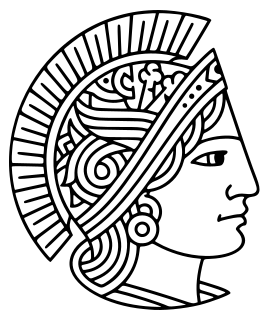
\includegraphics[scale=.12]{images/TUD}%
  %there must be an empty line above this line - otherwise some unwanted space is added between the university and the country (I do not know why;( )
}

\logo{
       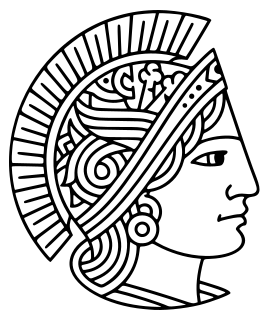
\includegraphics[scale=.03]{images/TUD}%
}

\date{\today}

%\AtBeginSection[]
%{
% \begin{frame}<beamer>
% \frametitle{Inhaltsverzeichnis}
% \tableofcontents[currentsection]
% \end{frame}
%}

%-------------------------------------------------------
% THE BODY OF THE PRESENTATION
%-------------------------------------------------------

\begin{document}

%-------------------------------------------------------
% THE TITLEPAGE
%-------------------------------------------------------

{\1
\begin{frame}[plain, noframenumbering] 
  \titlepage 
\end{frame}}

\begin{frame}{Outline}{}
\tableofcontents
\end{frame}

\AtBeginSection[]
{
	\begin{frame}{Outline}
		\tableofcontents[currentsection]
	\end{frame}
}

%-------------------------------------------------------
\section{Introduction and Motivation}
%-------------------------------------------------------

\begin{frame}{Introduction and Motivation}
	\centering
	\begin{figure}
		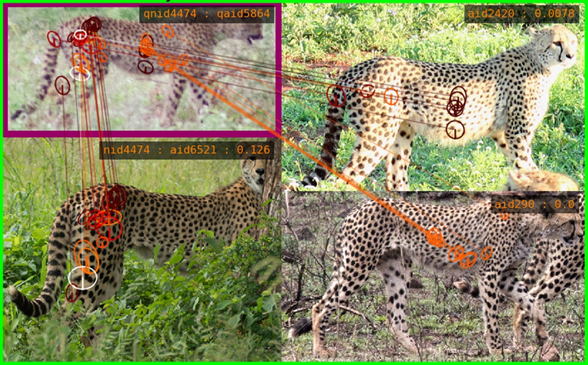
\includegraphics[width=.8\linewidth,height=.8\textheight,keepaspectratio]{images/biometrics.png}
		\caption{Animal Biometrics Example}
	\end{figure}
\end{frame}

%-------------------------------------------------------
\section{Problem 1: Classification of Species}
%-------------------------------------------------------
\subsection{Data Set}
%-------------------------------------------------------

\begin{frame}{Data Set}
	\begin{minipage}[c]{0.48\linewidth}
		\centering
		\begin{figure}
			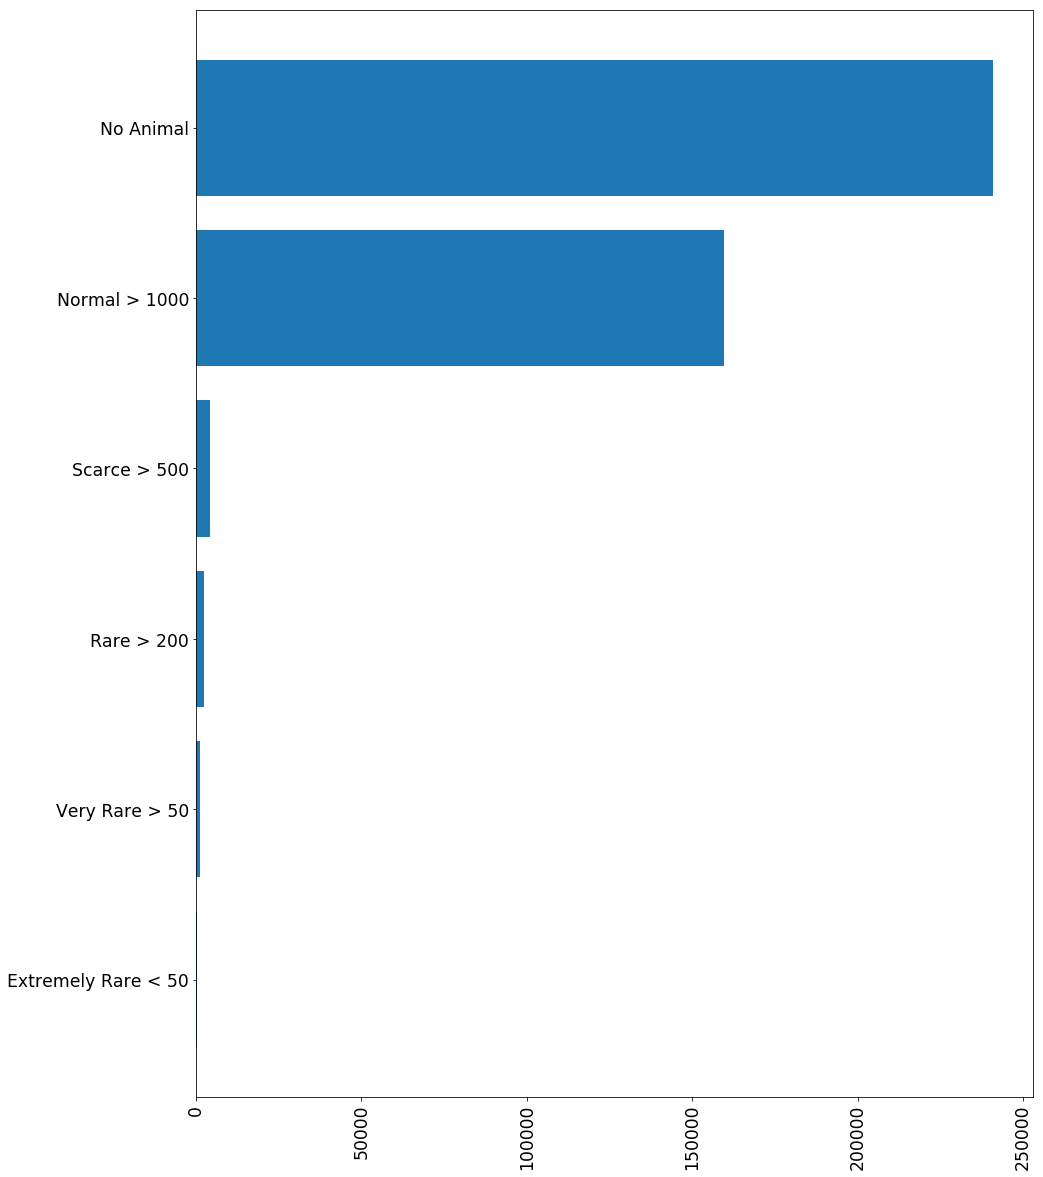
\includegraphics[width=\linewidth,height=.8\textheight,keepaspectratio]{images/Data_dist_sorted_reduced_v2.png}
			\caption{Reduced data distribution of species data set}
		\end{figure}
	\end{minipage}
	\hfill
	\begin{minipage}[c]{0.48\linewidth}
	\begin{itemize}
		\item Unbalanced data distribution (3 to 190k images per class)
		\item 87 classes/individuals
		\item Low quality images from camera traps
	\end{itemize}

	\end{minipage}
\end{frame}

%-------------------------------------------------------

\begin{frame}{Good Example Images}		
	\centering
	\begin{minipage}[c]{0.48\linewidth}
		\begin{figure}
			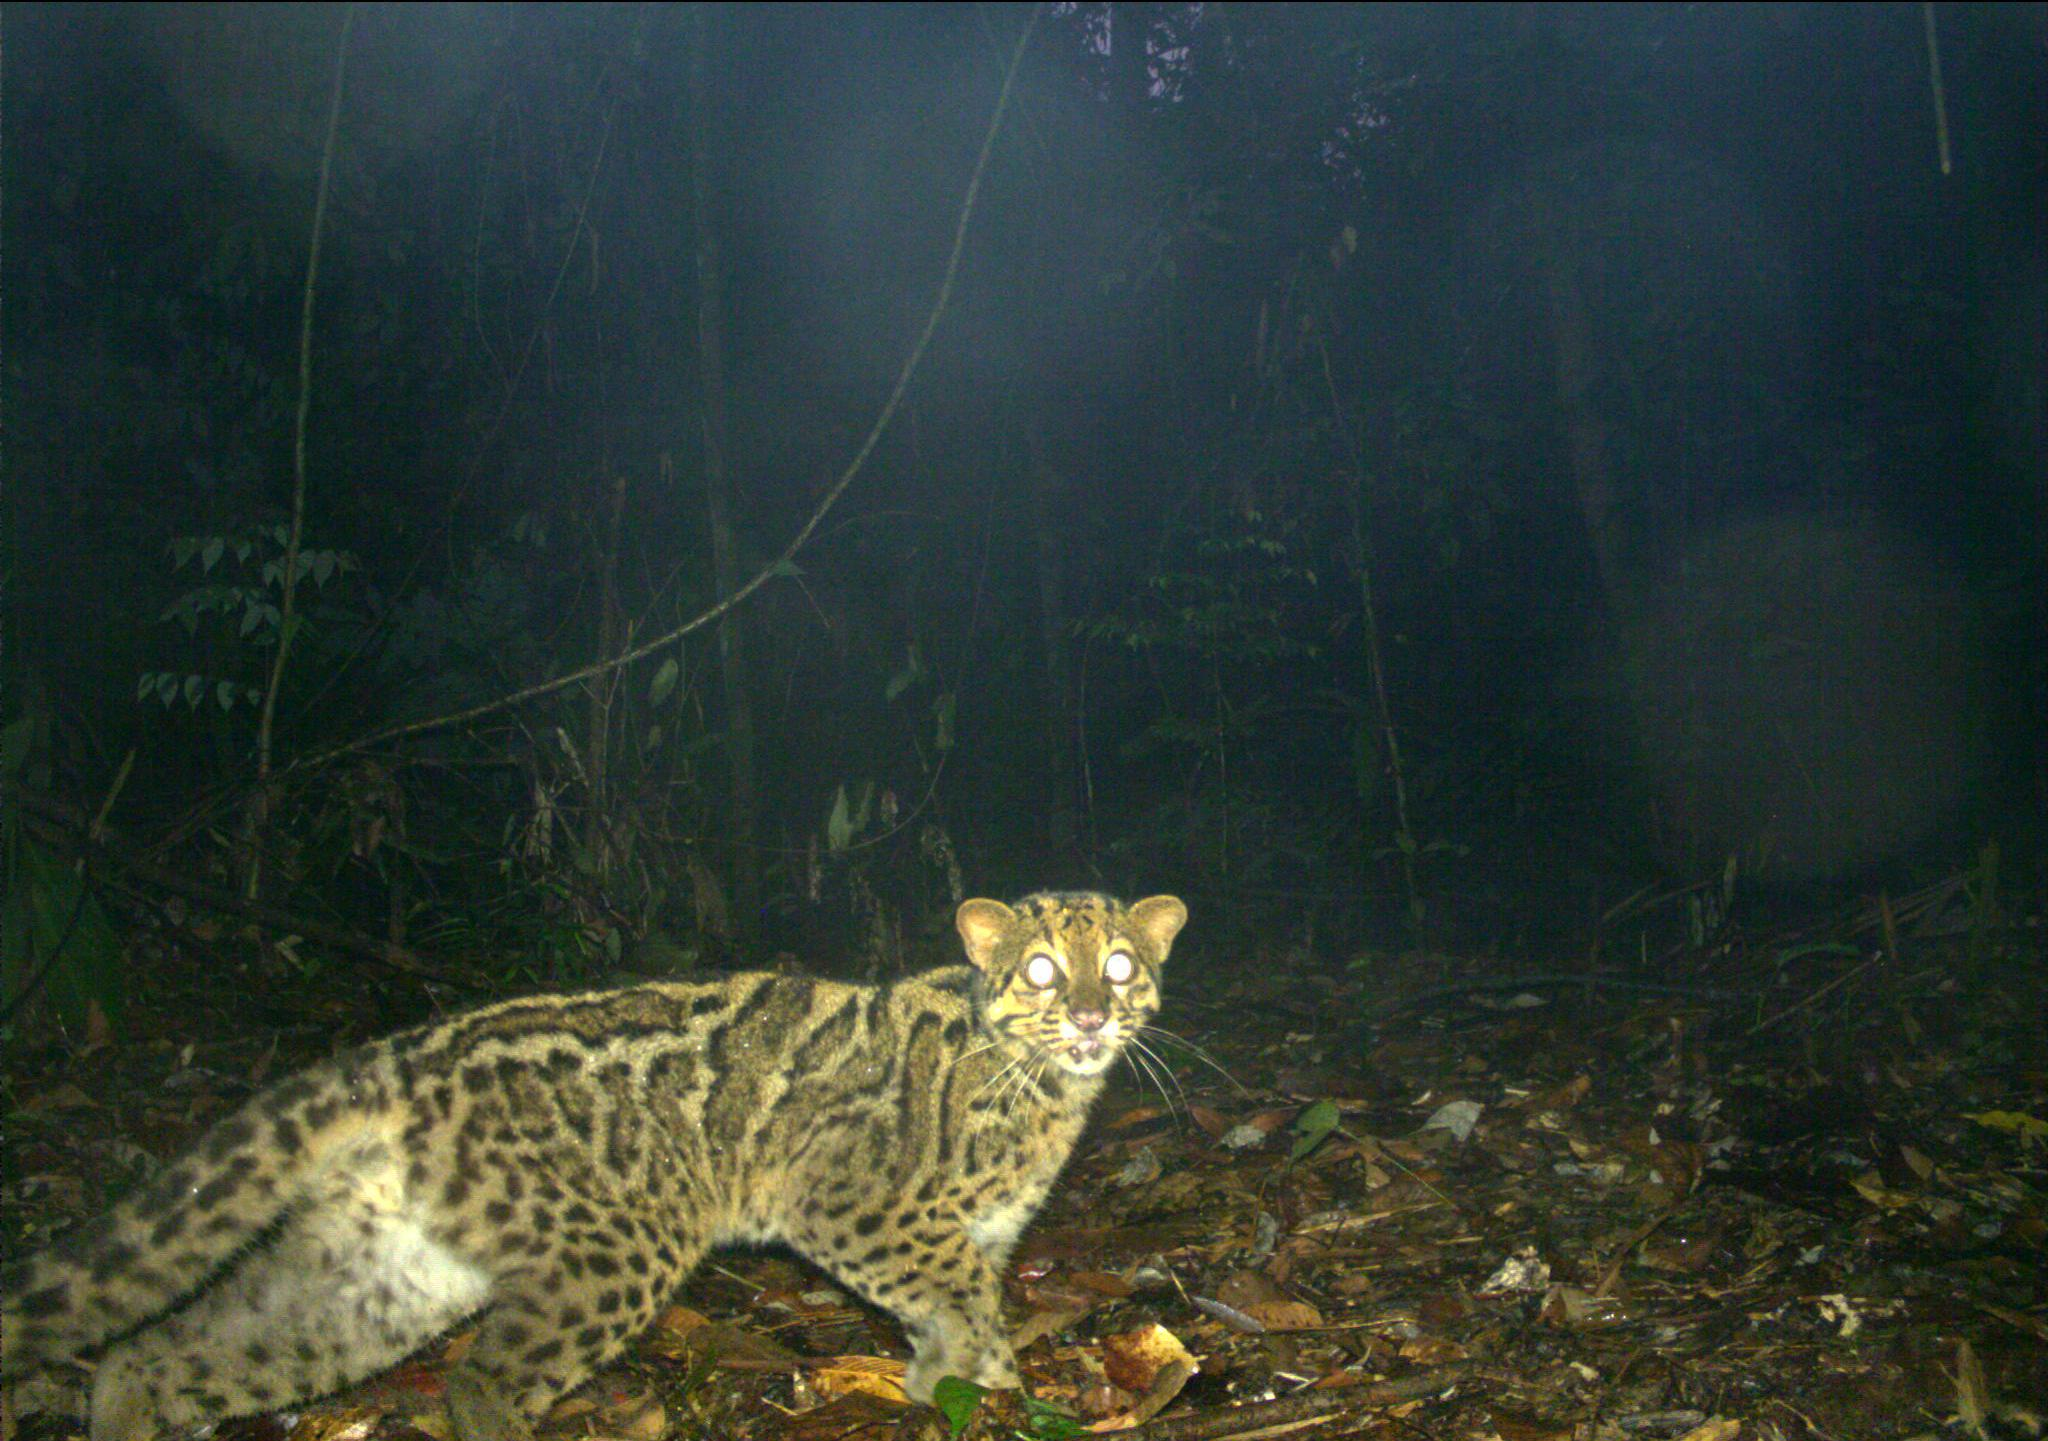
\includegraphics[width=\linewidth,height=\textheight,keepaspectratio]{images/example_marbled_cat.JPG}
			\caption{Marbled Cat}
		\end{figure}
	\end{minipage}
	\hfill
	\begin{minipage}[c]{0.48\linewidth}
		\begin{figure}
			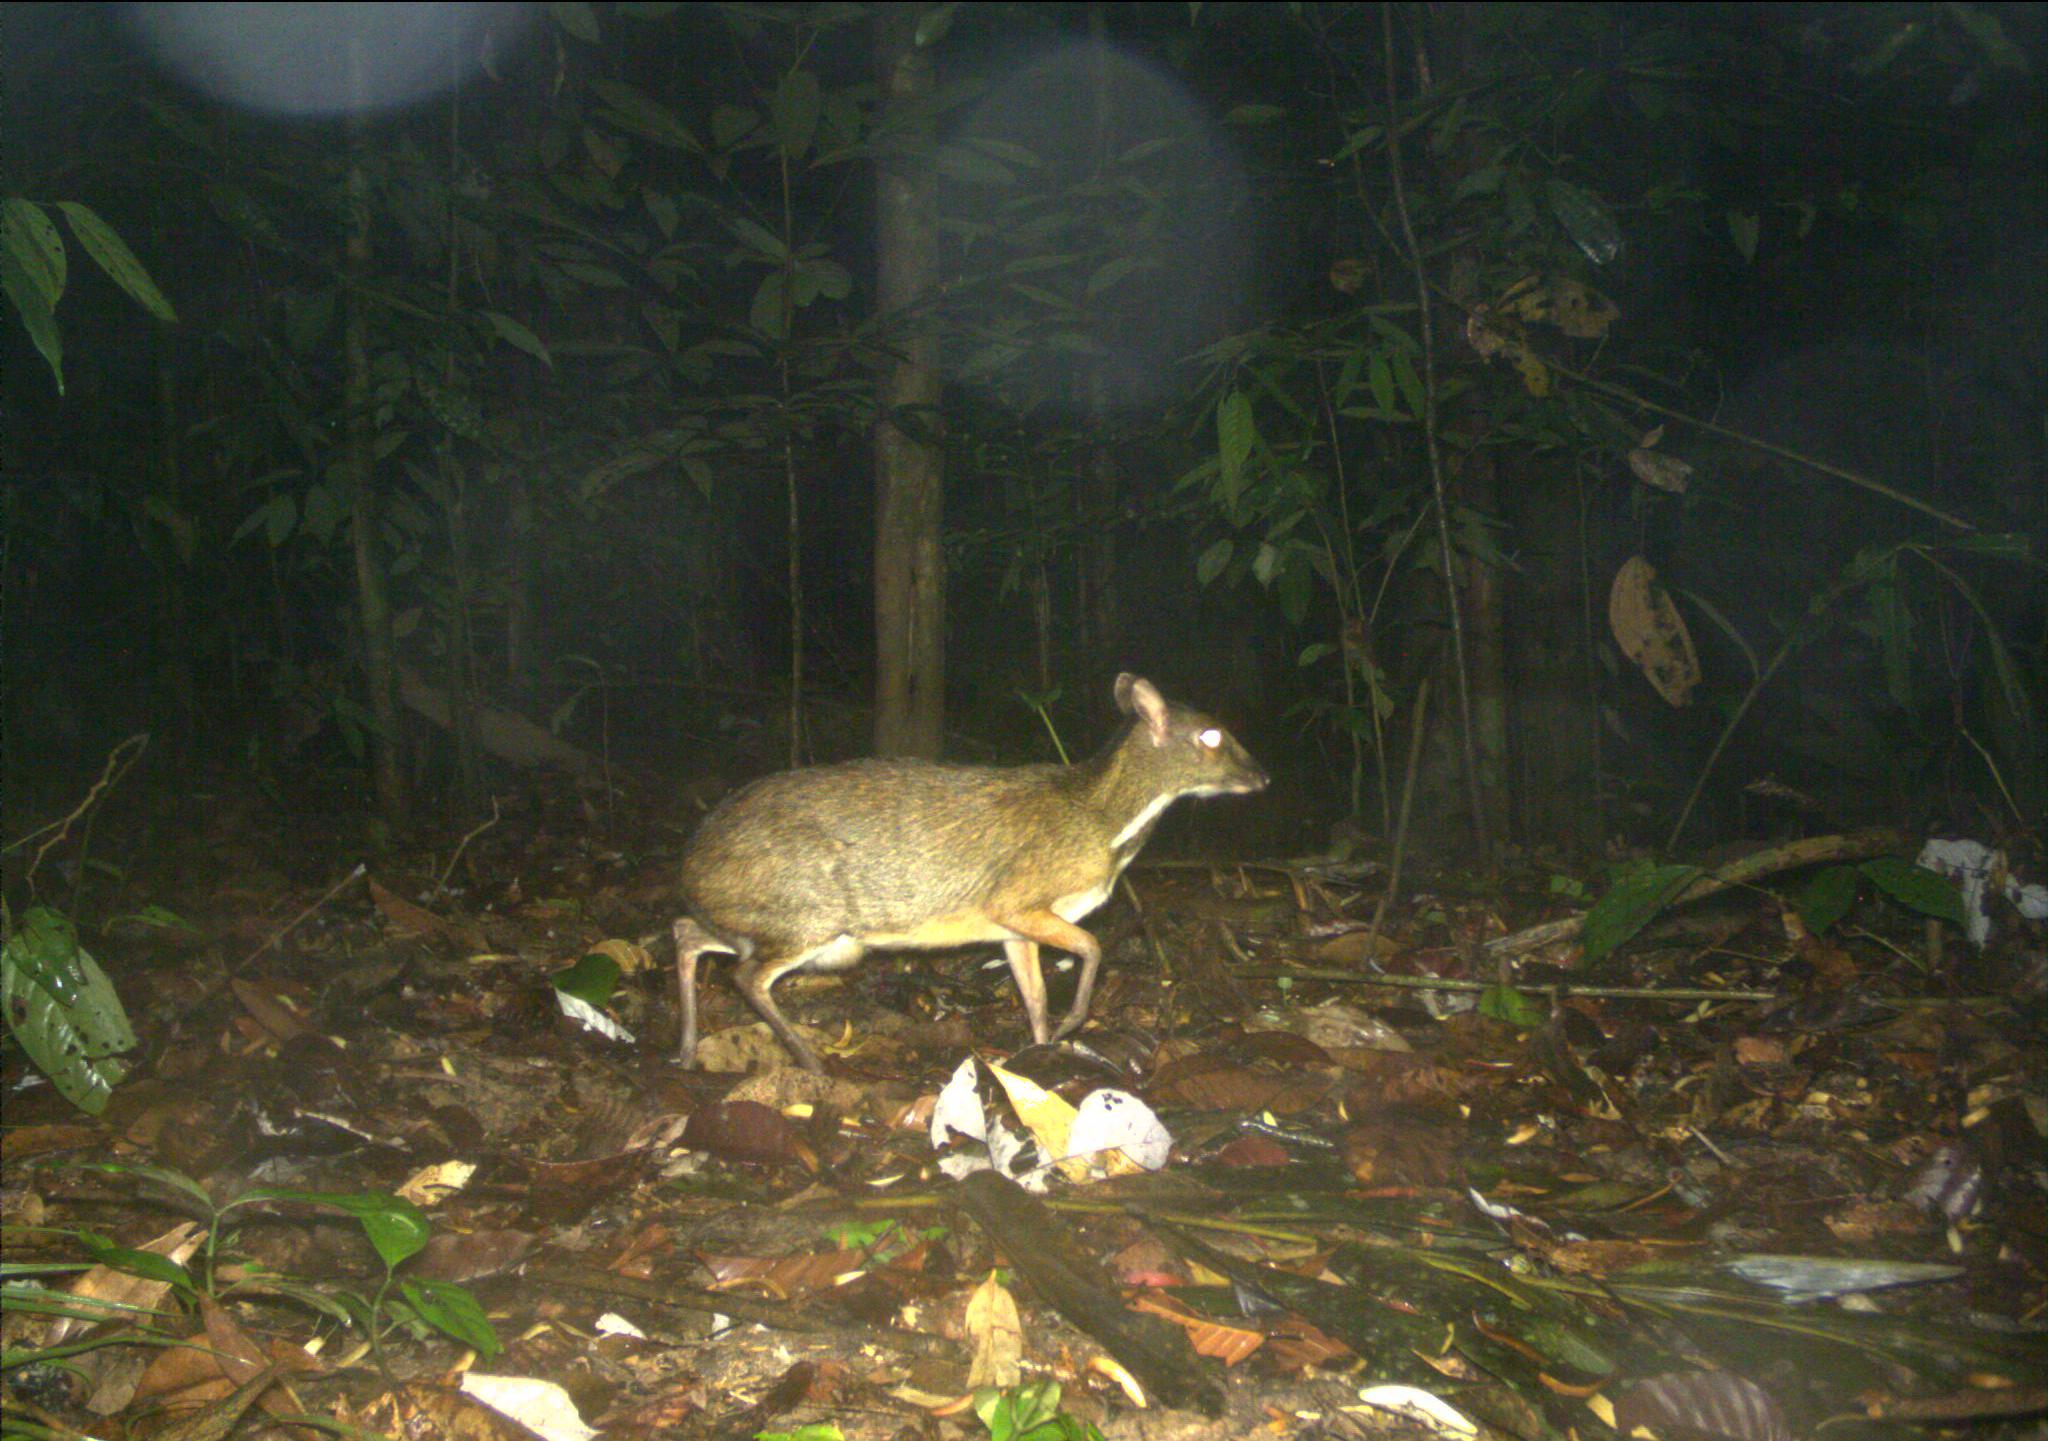
\includegraphics[width=\linewidth,height=.8\textheight,keepaspectratio]{images/example_mouse_deer.JPG}
			\caption{Mouse Deer}
		\end{figure}
	\end{minipage}
\end{frame}

%-------------------------------------------------------

\begin{frame}{Bad Example Images}		
	\centering
	\begin{minipage}[c]{0.48\linewidth}
		\begin{figure}
			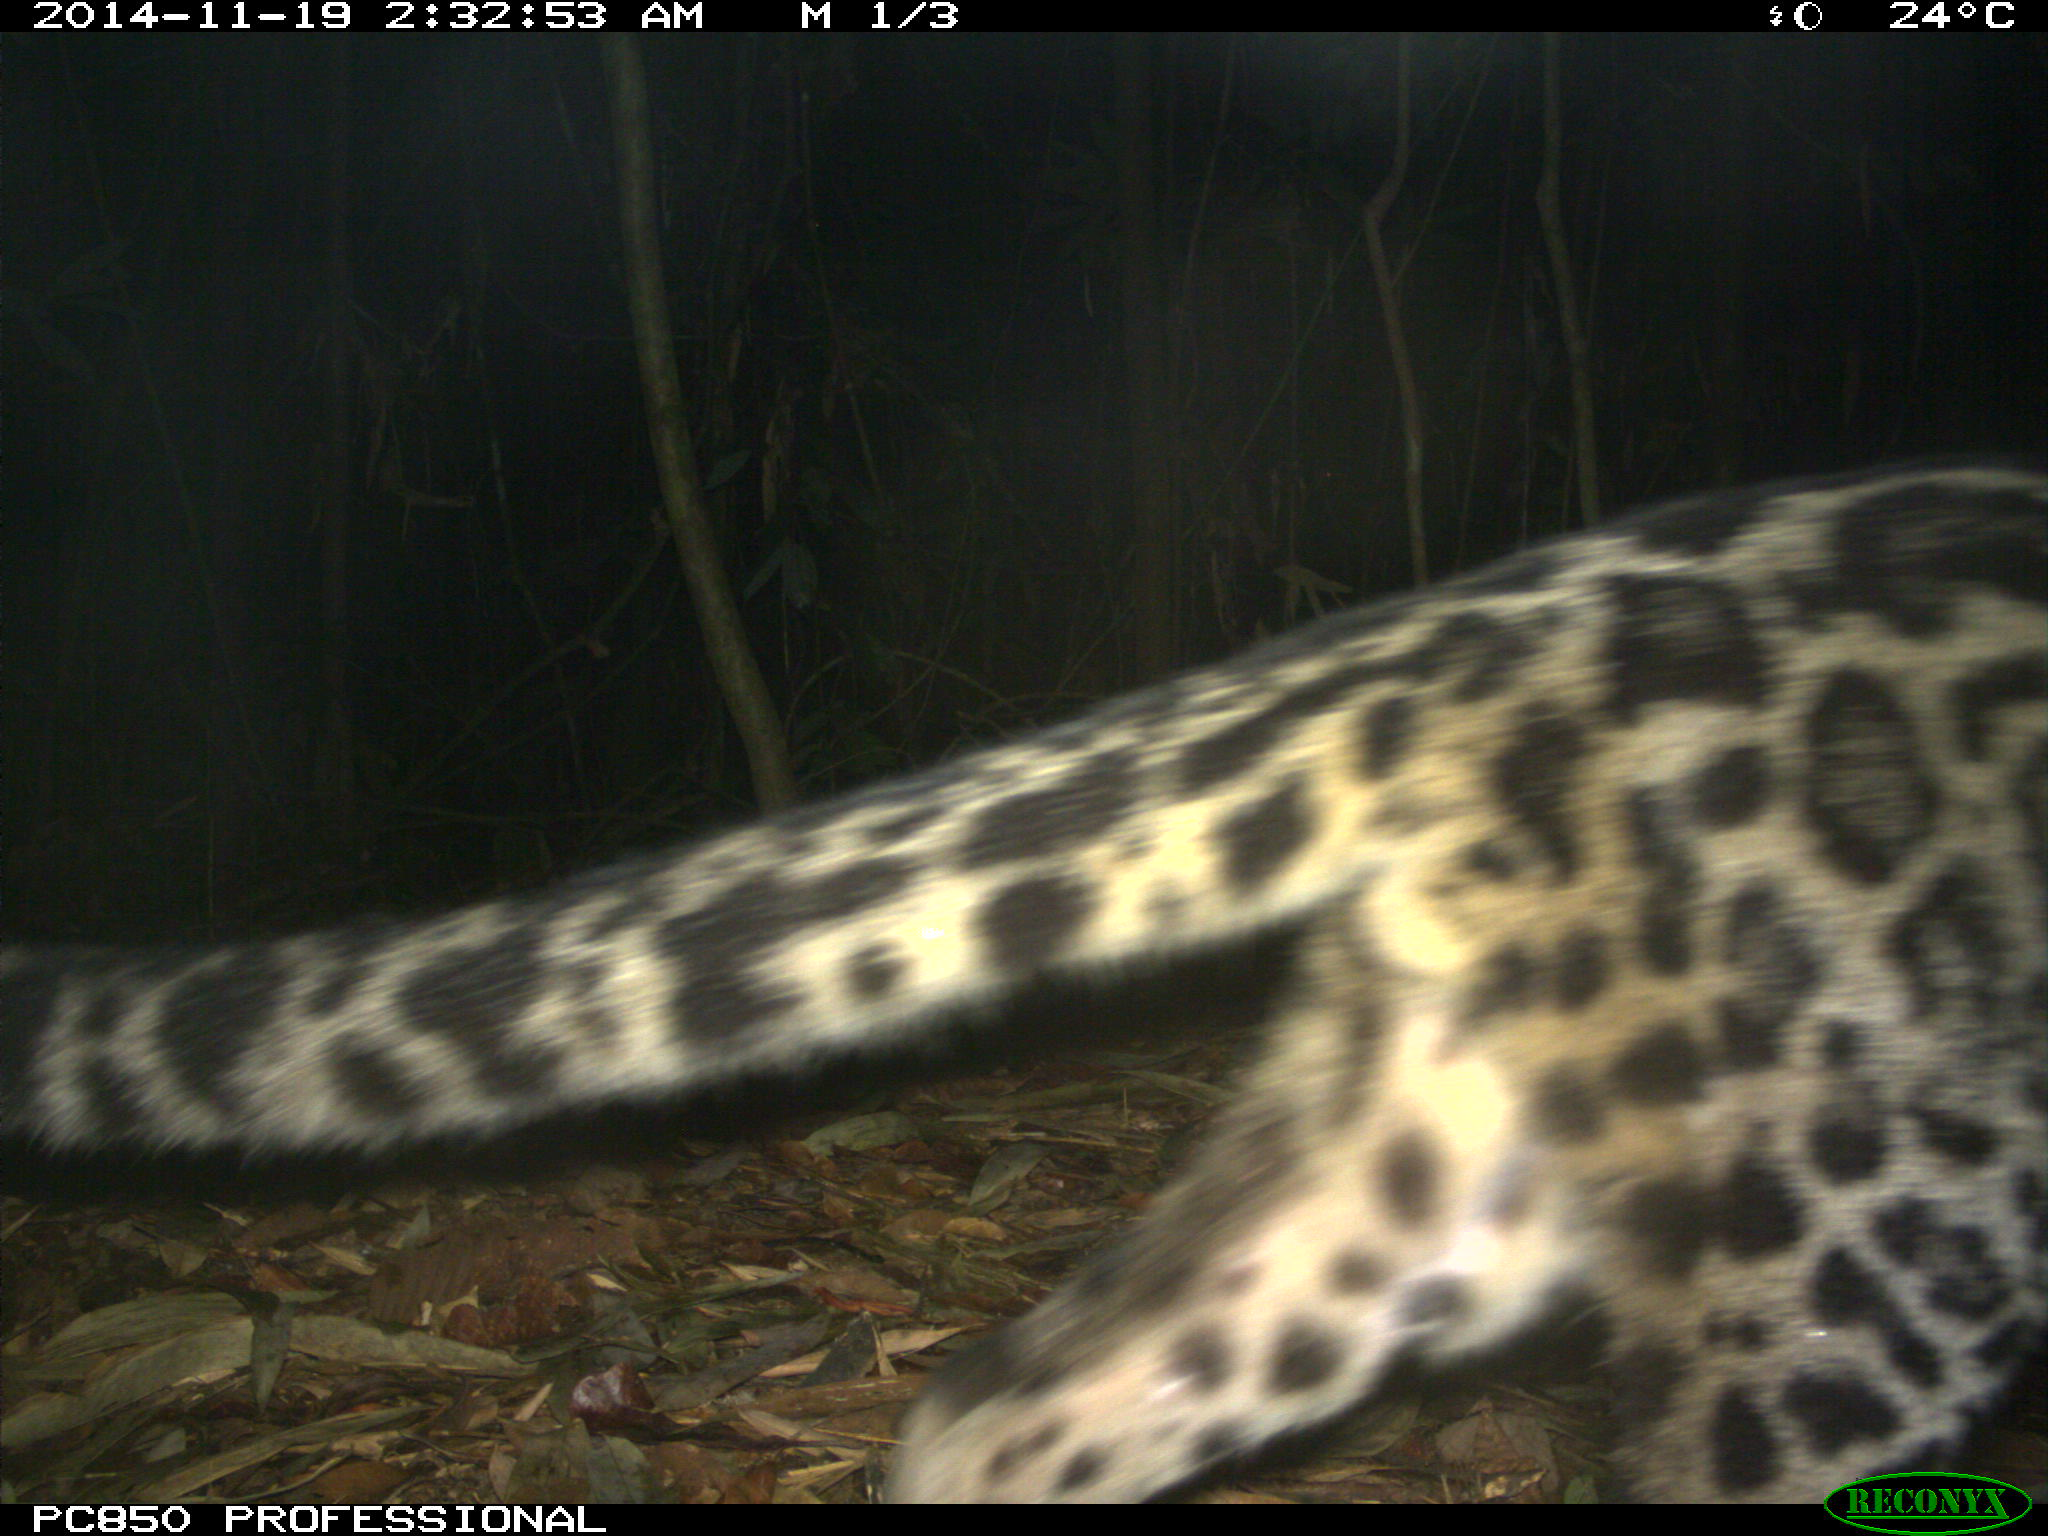
\includegraphics[width=.95\linewidth,keepaspectratio]{images/example_bad_DFR_7_female.JPG}
			\hfill
			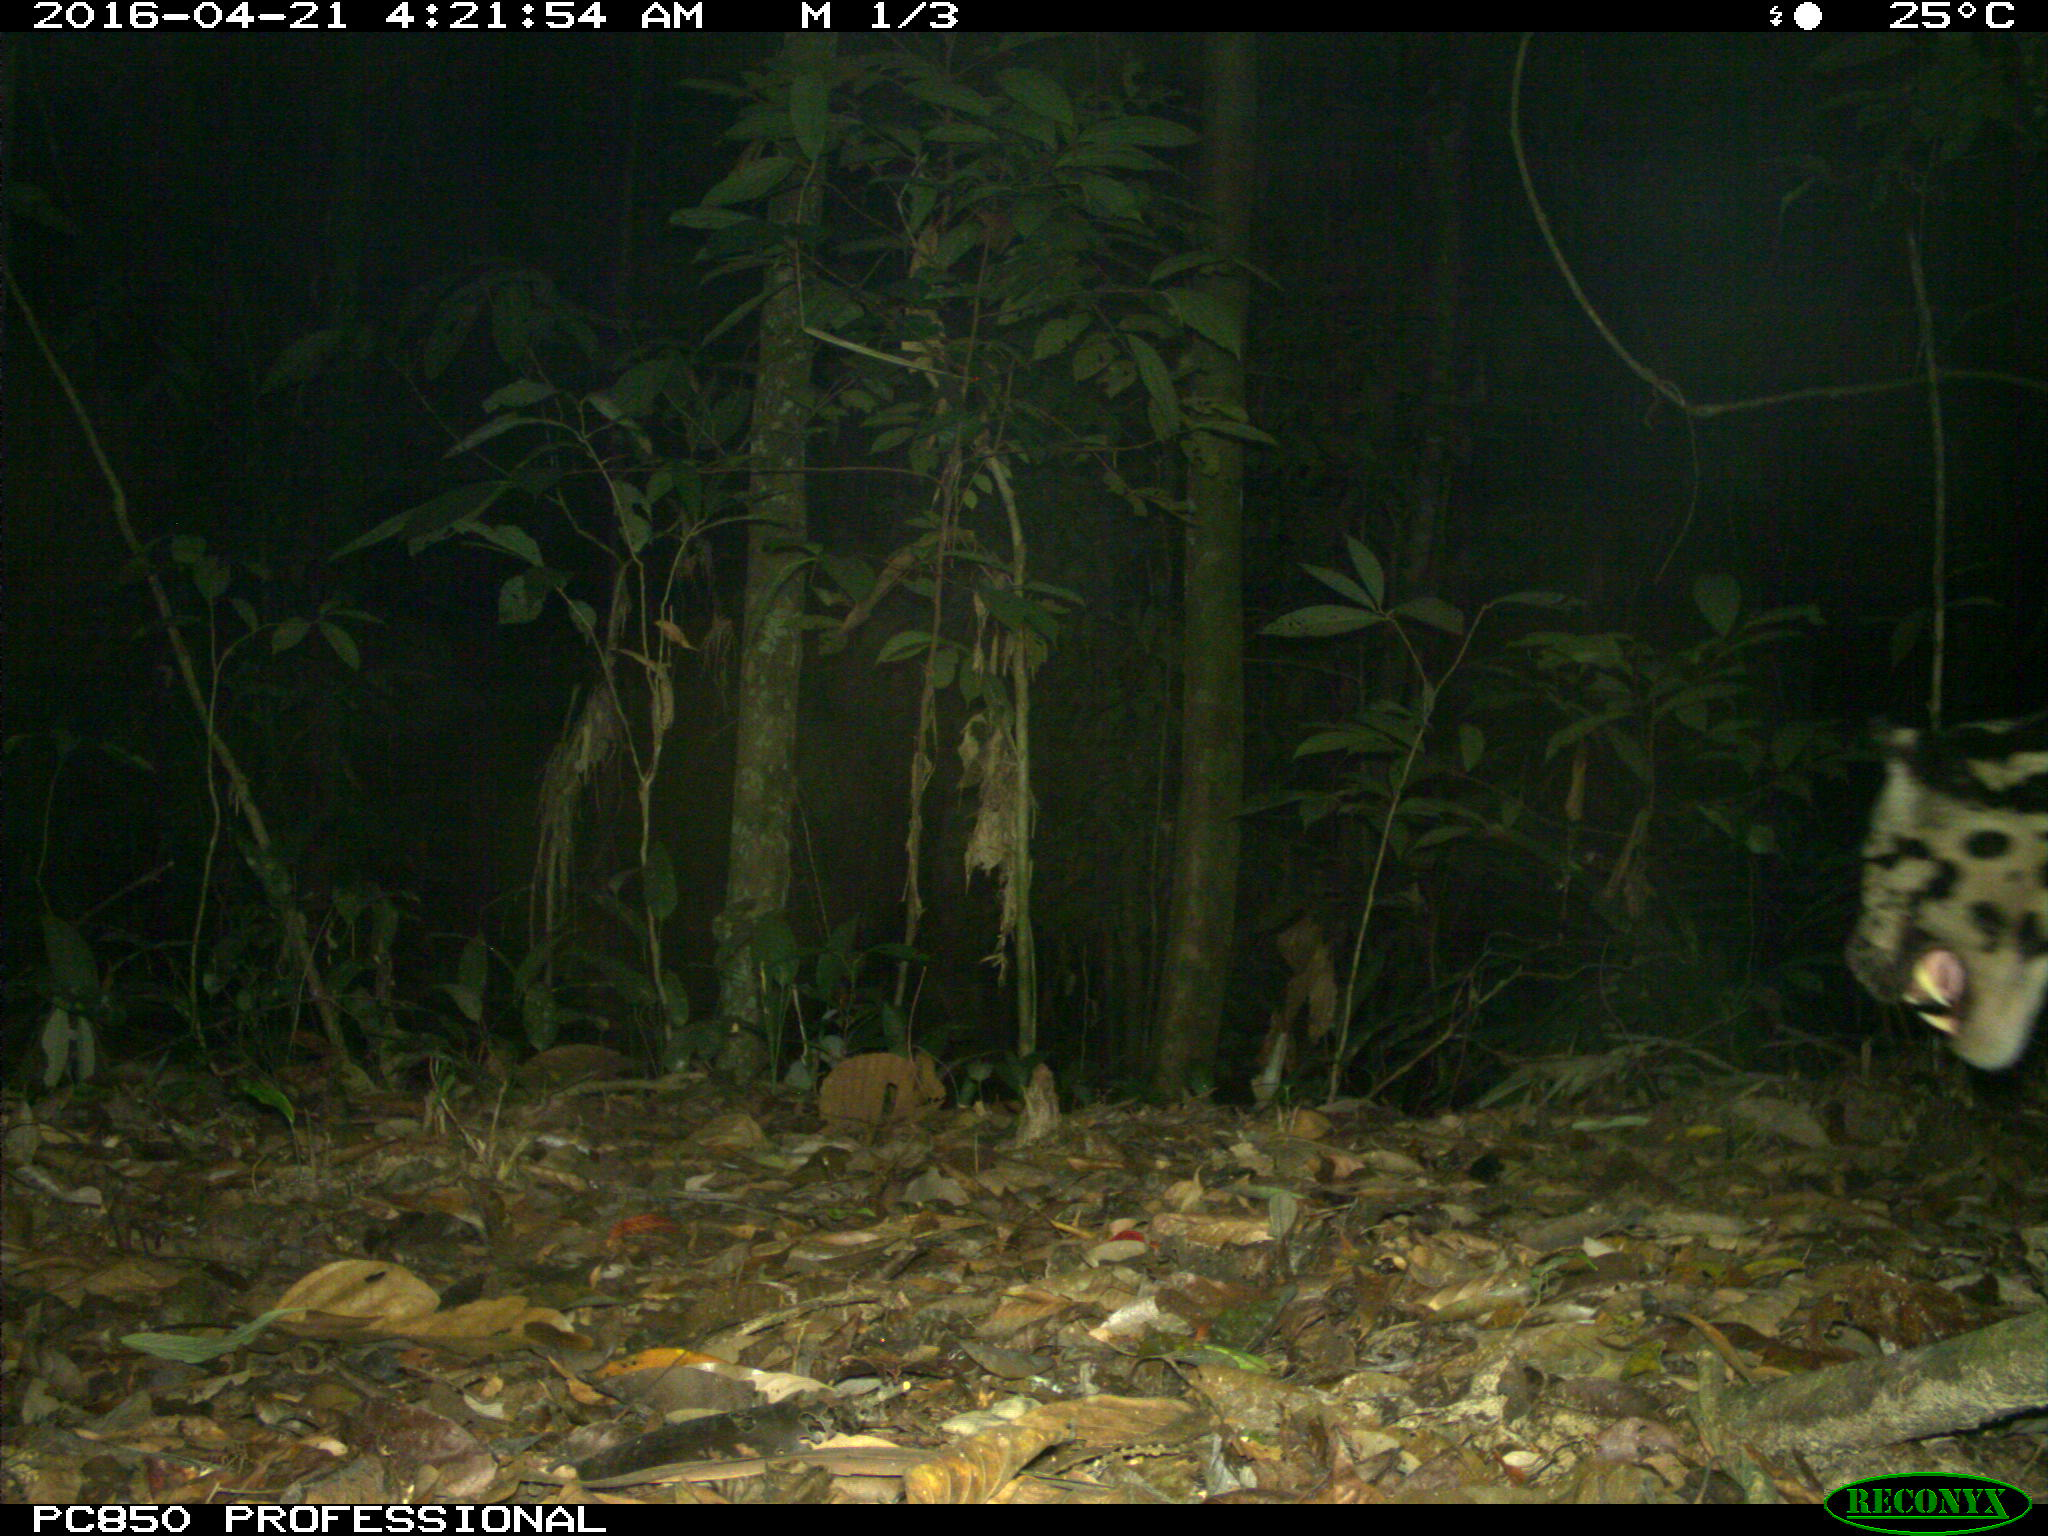
\includegraphics[width=.95\linewidth,keepaspectratio]{images/example_bad_KFR_3_Male.JPG}
		\end{figure}
	\end{minipage}
	\hfill
	\begin{minipage}[c]{0.48\linewidth}
		\begin{figure}
			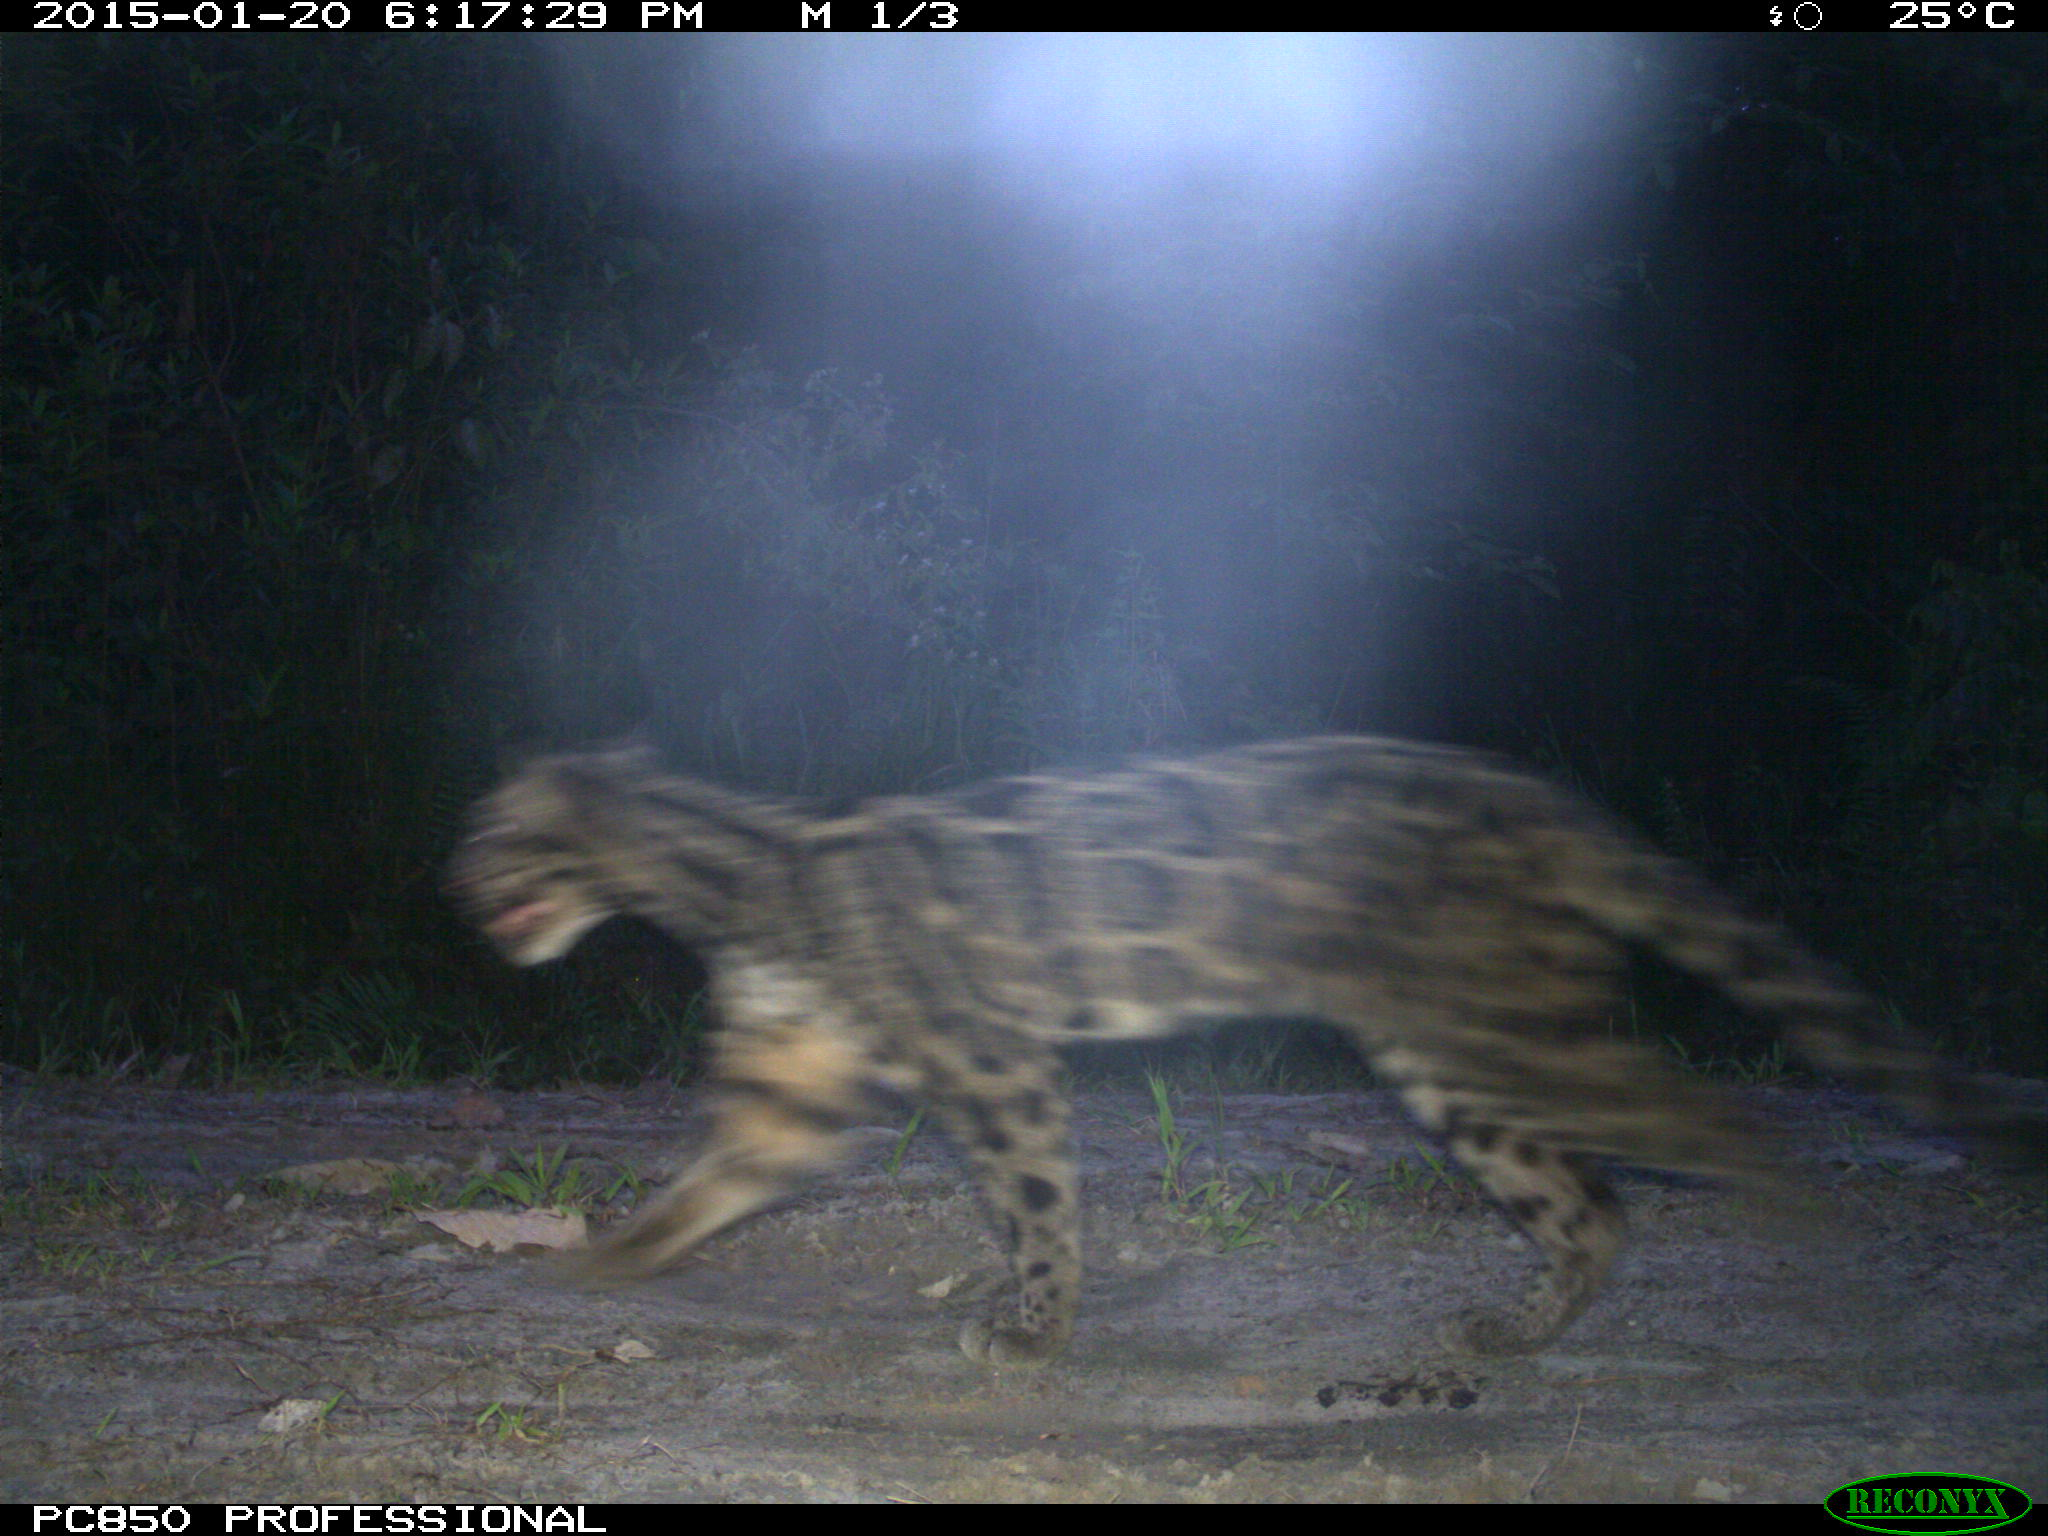
\includegraphics[width=\linewidth,height=\textheight,keepaspectratio]{images/example_bad_DFR_9_female.JPG}
			\caption{Bad quality training images}	
		\end{figure}
	\end{minipage}
\end{frame}

%-------------------------------------------------------
\subsection{Architecture}
%-------------------------------------------------------

\begin{frame}{Architecture}
	\begin{figure}
		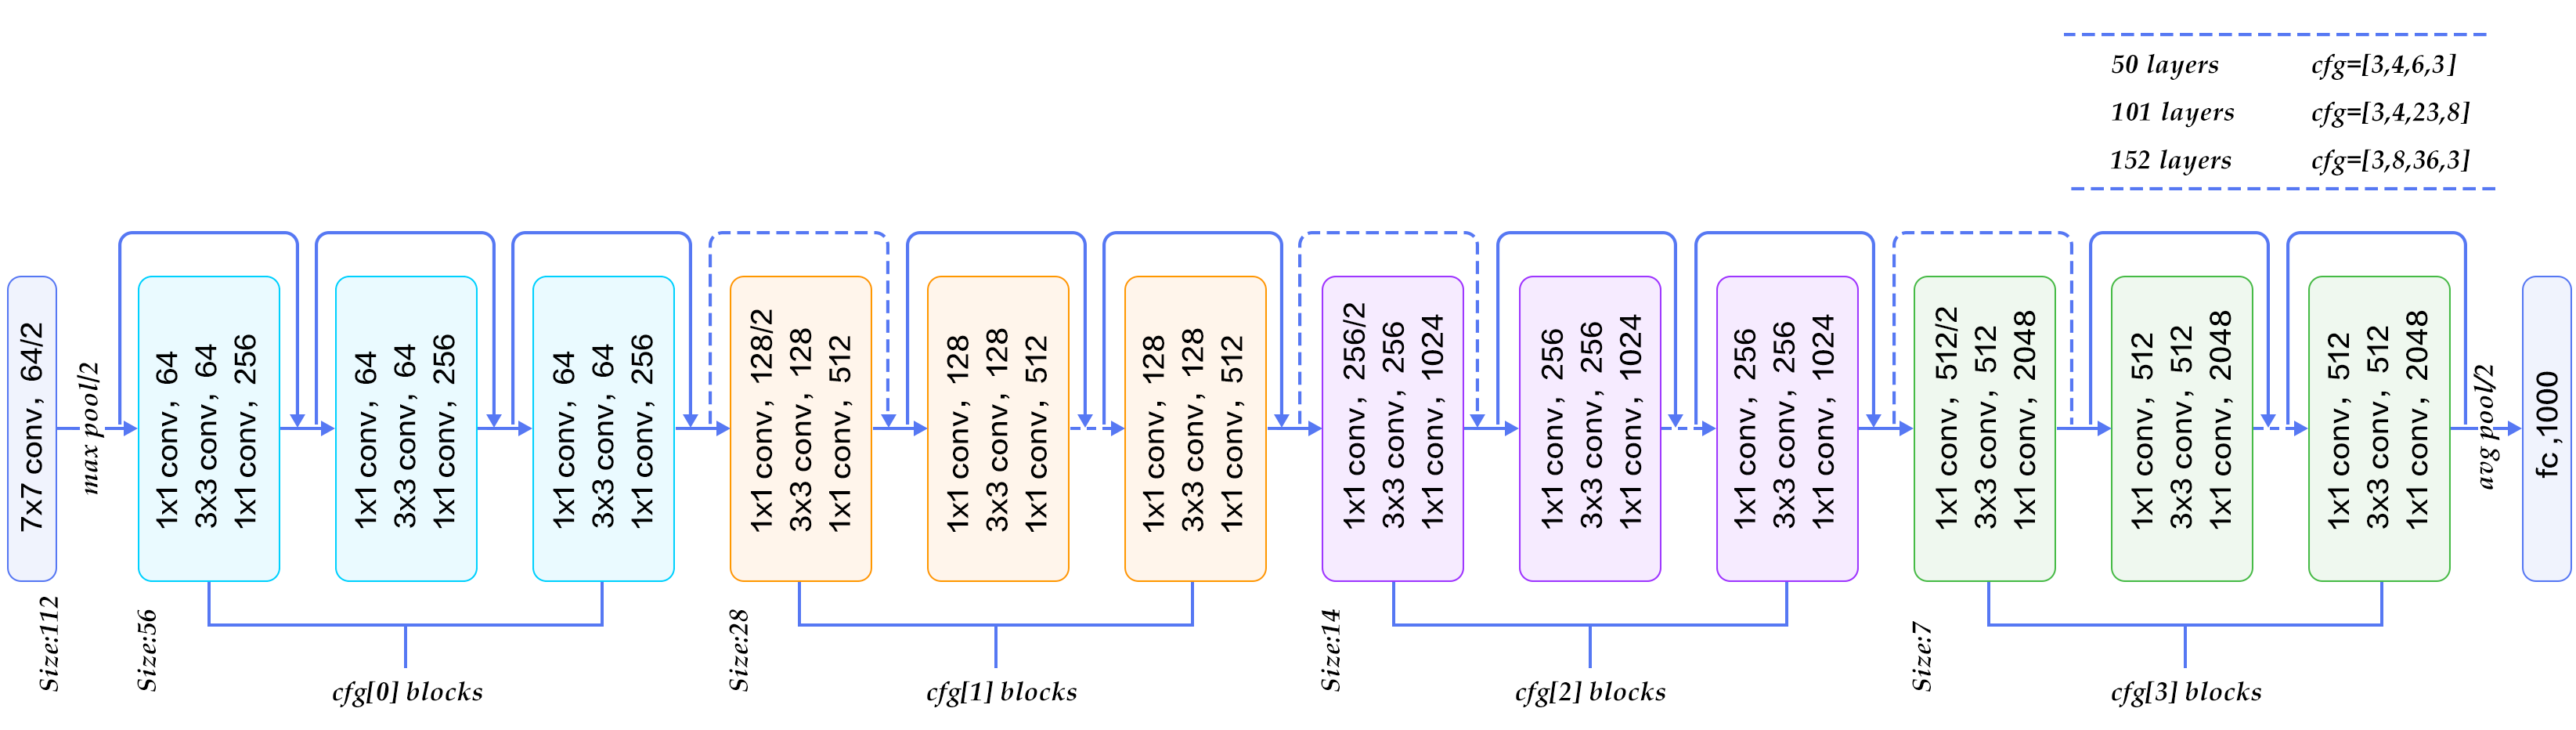
\includegraphics[width=\columnwidth]{images/resnet.png}
		\caption{ResNet Architecture\newline{} [\url{https://www.codeproject.com/Articles/1248963/Deep-Learning-using-Python-plus-Keras-Chapter-Re}]}
	\end{figure}

	\begin{itemize}
		\item ResNet-50 finetuning and from scratch
	\end{itemize}
\end{frame}

%-------------------------------------------------------
\subsection{Results}
%-------------------------------------------------------

\begin{frame}{Scores}
	\centering
	\begin{minipage}[r]{0.58\linewidth}
		\begin{figure}
			\makebox[\textwidth][l]{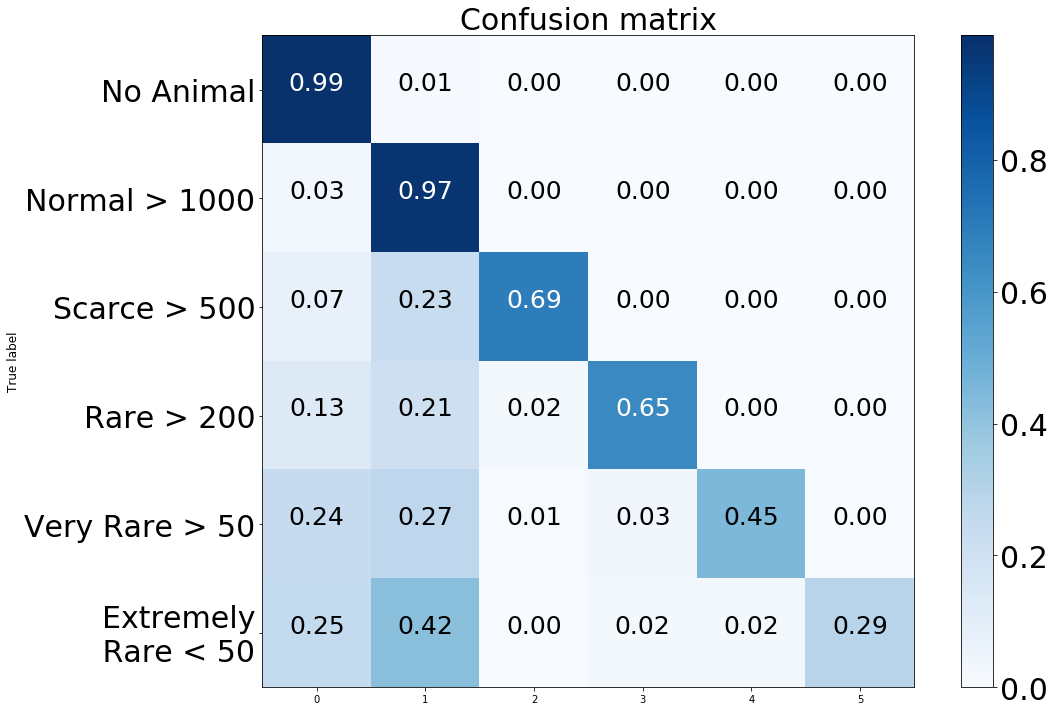
\includegraphics[width=\columnwidth]{images/conf_mat_large.png}}
			\hfill
			\hspace*{.5cm}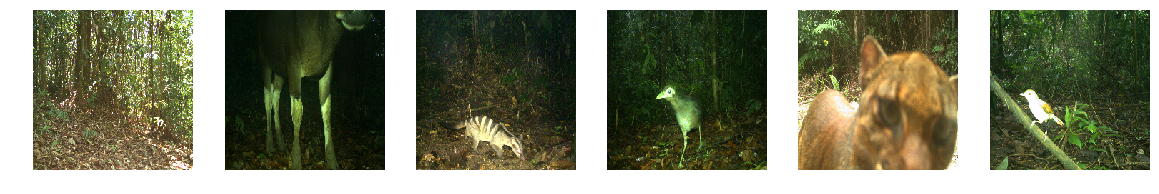
\includegraphics[width=.8\columnwidth]{images/images_below.png}
			\caption{Reduced confusion matrix for finetuned ResNet-50}
		\end{figure}
	\end{minipage}
	\begin{minipage}[c]{0.38\linewidth}
		\textbf{Test set:}
		\begin{itemize}
			\item Accuracy: $0.95$
			\item Avg. Precision: $0.95$      
			\item Avg. Recall: $0.95$
			\item Avg. F1-Score: $0.95$
		\end{itemize}
	\end{minipage}
\end{frame}

%-------------------------------------------------------

\begin{frame}{Training Process}
	\centering
	\begin{figure}
		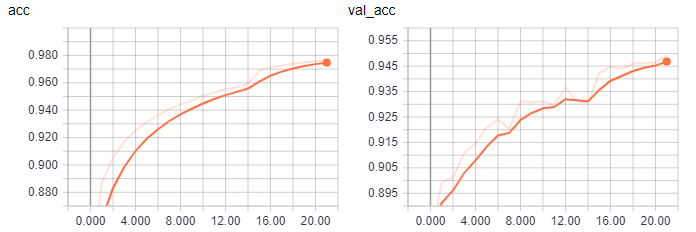
\includegraphics[width=.9\columnwidth,height=\textheight,keepaspectratio]{images/acc.png}
		\caption{Accuracy during Training}
	\end{figure}
\end{frame}

%-------------------------------------------------------

\begin{frame}{Positive Examples}
	\centering
	\begin{figure}
		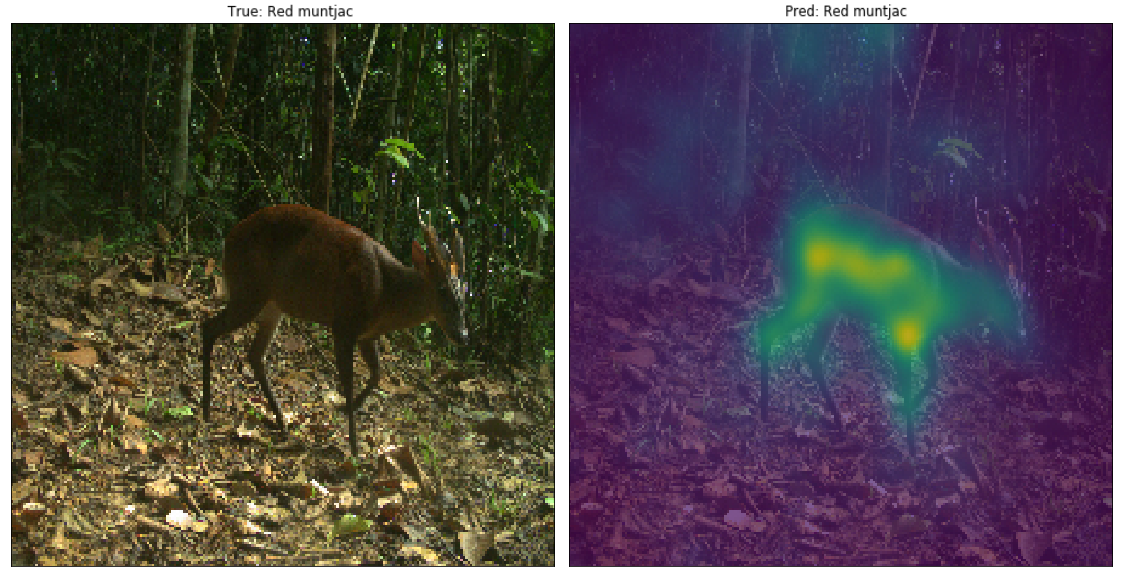
\includegraphics[width=\columnwidth]{images/Attention_right6.png}
		\caption{Correct attention and classification}
	\end{figure}
\end{frame}

%-------------------------------------------------------

\begin{frame}{Positive Examples}
	\centering
	\begin{figure}
		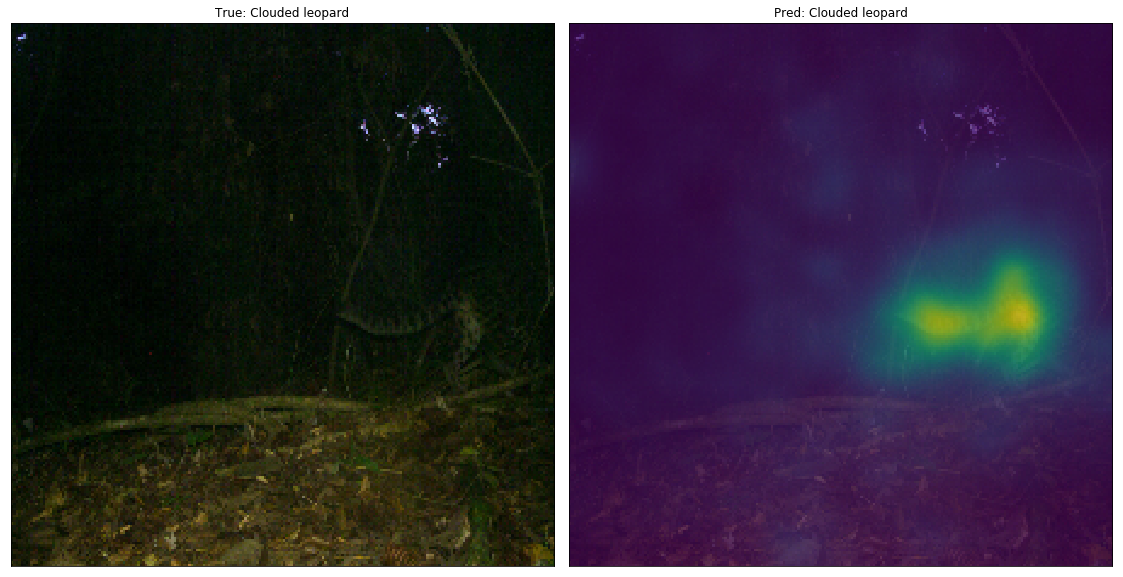
\includegraphics[width=\columnwidth]{images/Attention_right5.png}
		\caption{Correct attention and classification}
	\end{figure}
\end{frame}

%-------------------------------------------------------

\begin{frame}{Negative Examples}
	\centering
	\begin{figure}
		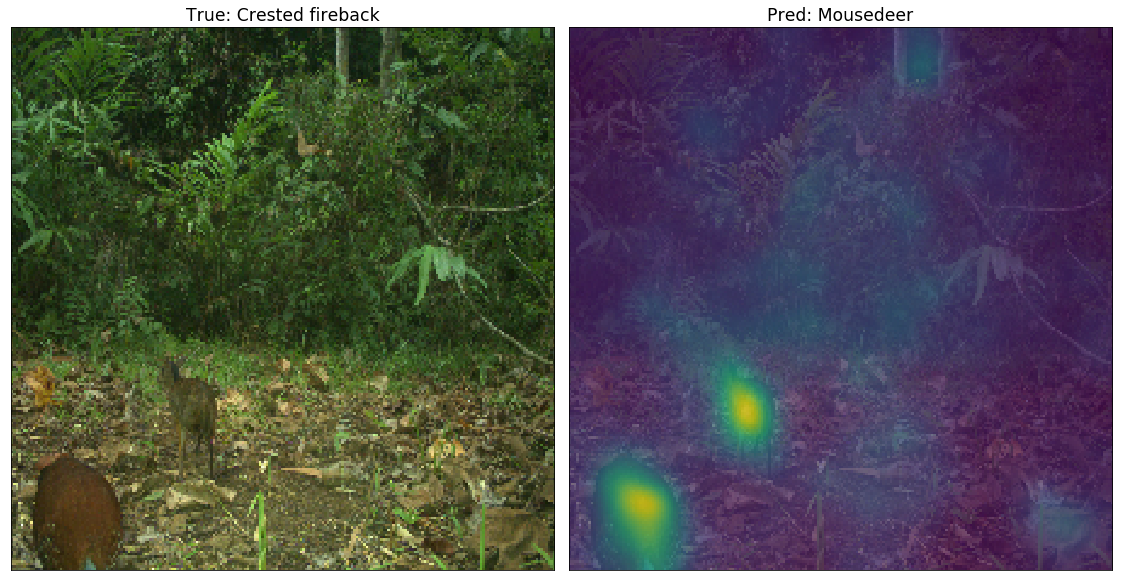
\includegraphics[width=\columnwidth]{images/Attention_wrong_right.png}
		\caption{Noisy labels}
	\end{figure}
\end{frame}

%-------------------------------------------------------

\begin{frame}{Negative Examples}
	\centering
	\begin{figure}
		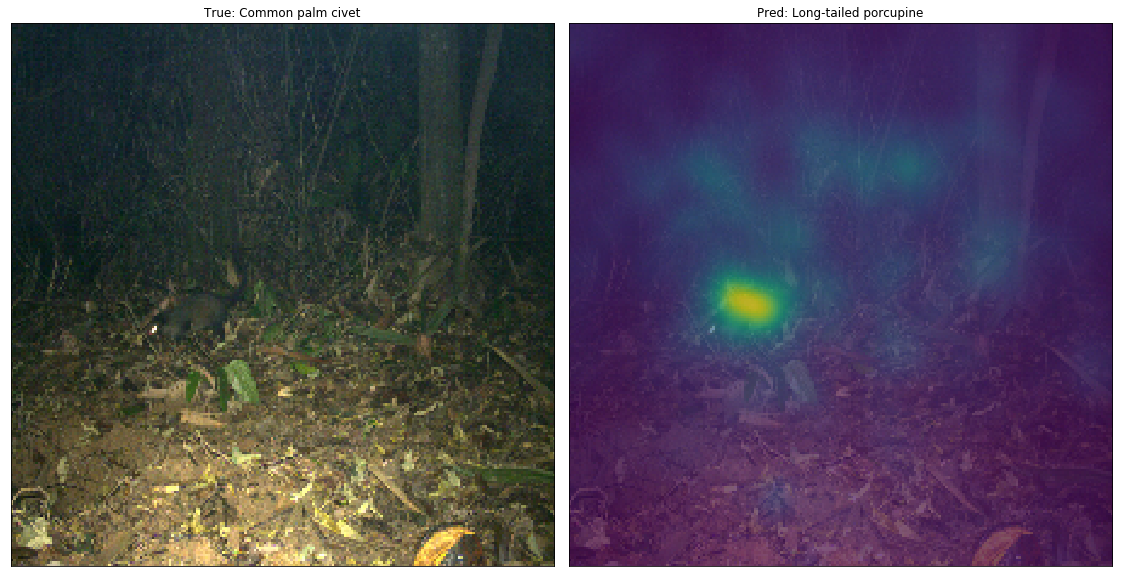
\includegraphics[width=\columnwidth]{images/Attention_wrong.png}
		\caption{Correct Attention, wrong label}
	\end{figure}
\end{frame}

%-------------------------------------------------------

\begin{frame}{Negative Examples}
	\centering
	\begin{figure}
		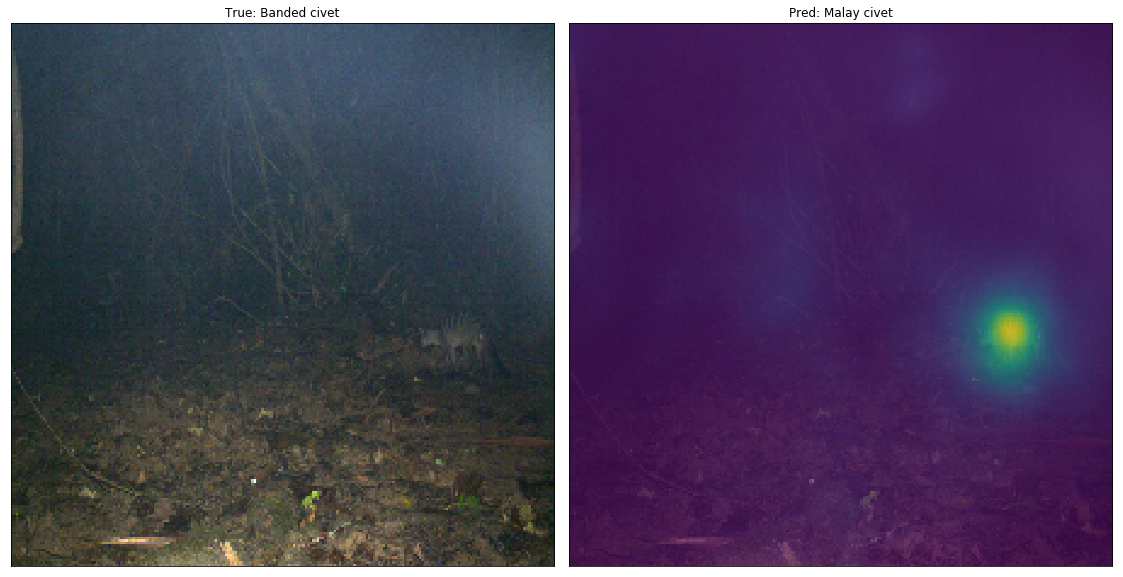
\includegraphics[width=\columnwidth]{images/mismatch.png}
		\caption{Mismatch because of class similarity}
	\end{figure}
\end{frame}

%-------------------------------------------------------
\section{Problem 2: Classification of Individuals}
%-------------------------------------------------------
\subsection{Data Set}
%-------------------------------------------------------
\begin{frame}{Data Set}
	\begin{minipage}[c]{0.48\linewidth}
		\centering
		\begin{figure}
			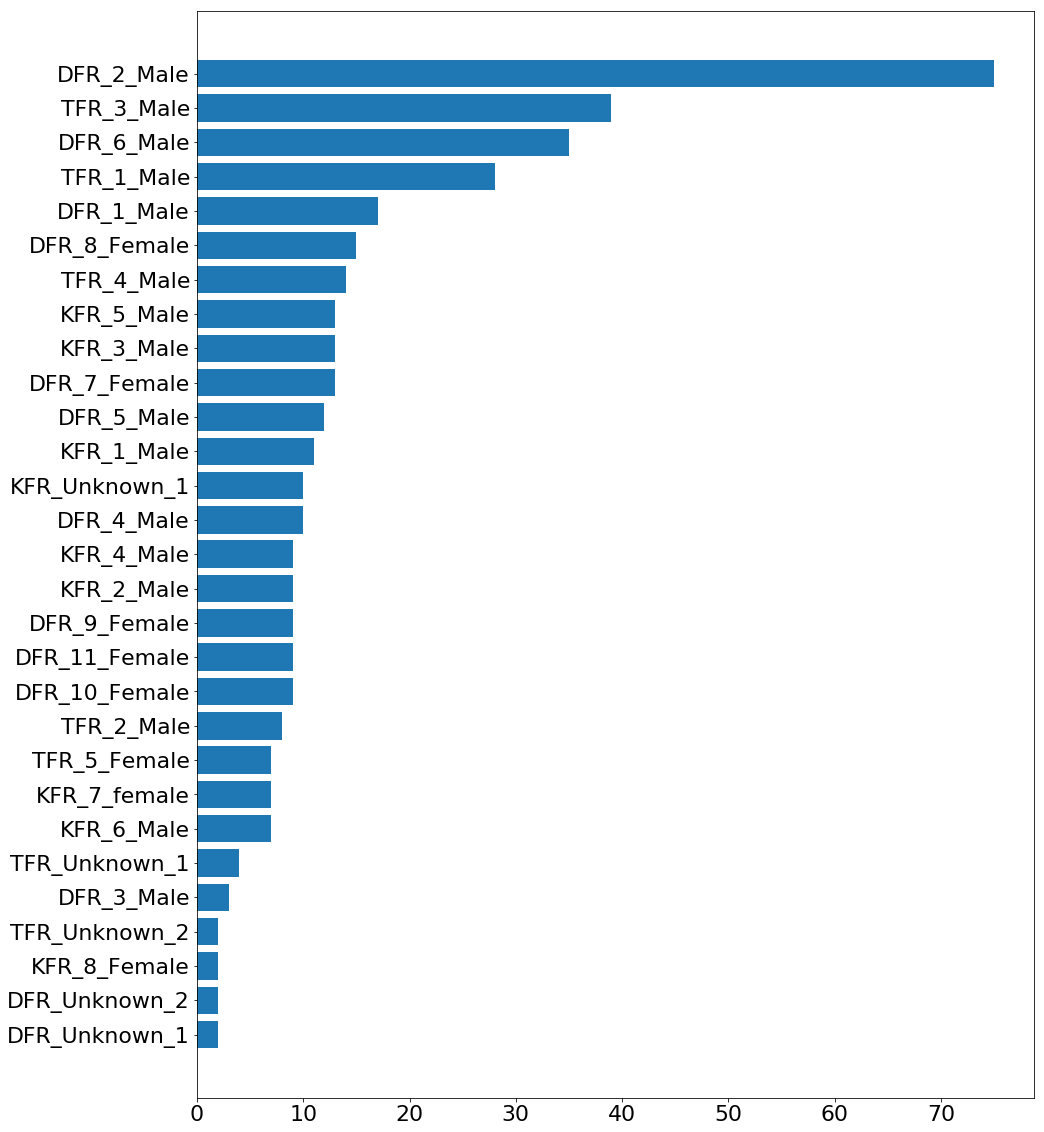
\includegraphics[width=\linewidth,height=.8\textheight,keepaspectratio]{images/Data_dist_leo_v2.png}
			\caption{Data distribution of individuals data set}
		\end{figure}
	\end{minipage}
	\hfill
	\begin{minipage}[c]{0.48\linewidth}
		\begin{itemize}
			\item Unbalanced data distribution (3 to 99 images per class)
			\item 29 classes/individuals
			\item Low quality images from camera traps
		\end{itemize}
	\end{minipage}
\end{frame}

%-------------------------------------------------------

\begin{frame}{Good Example Images}		
	\centering
	\begin{minipage}[c]{0.48\linewidth}
		\begin{figure}
			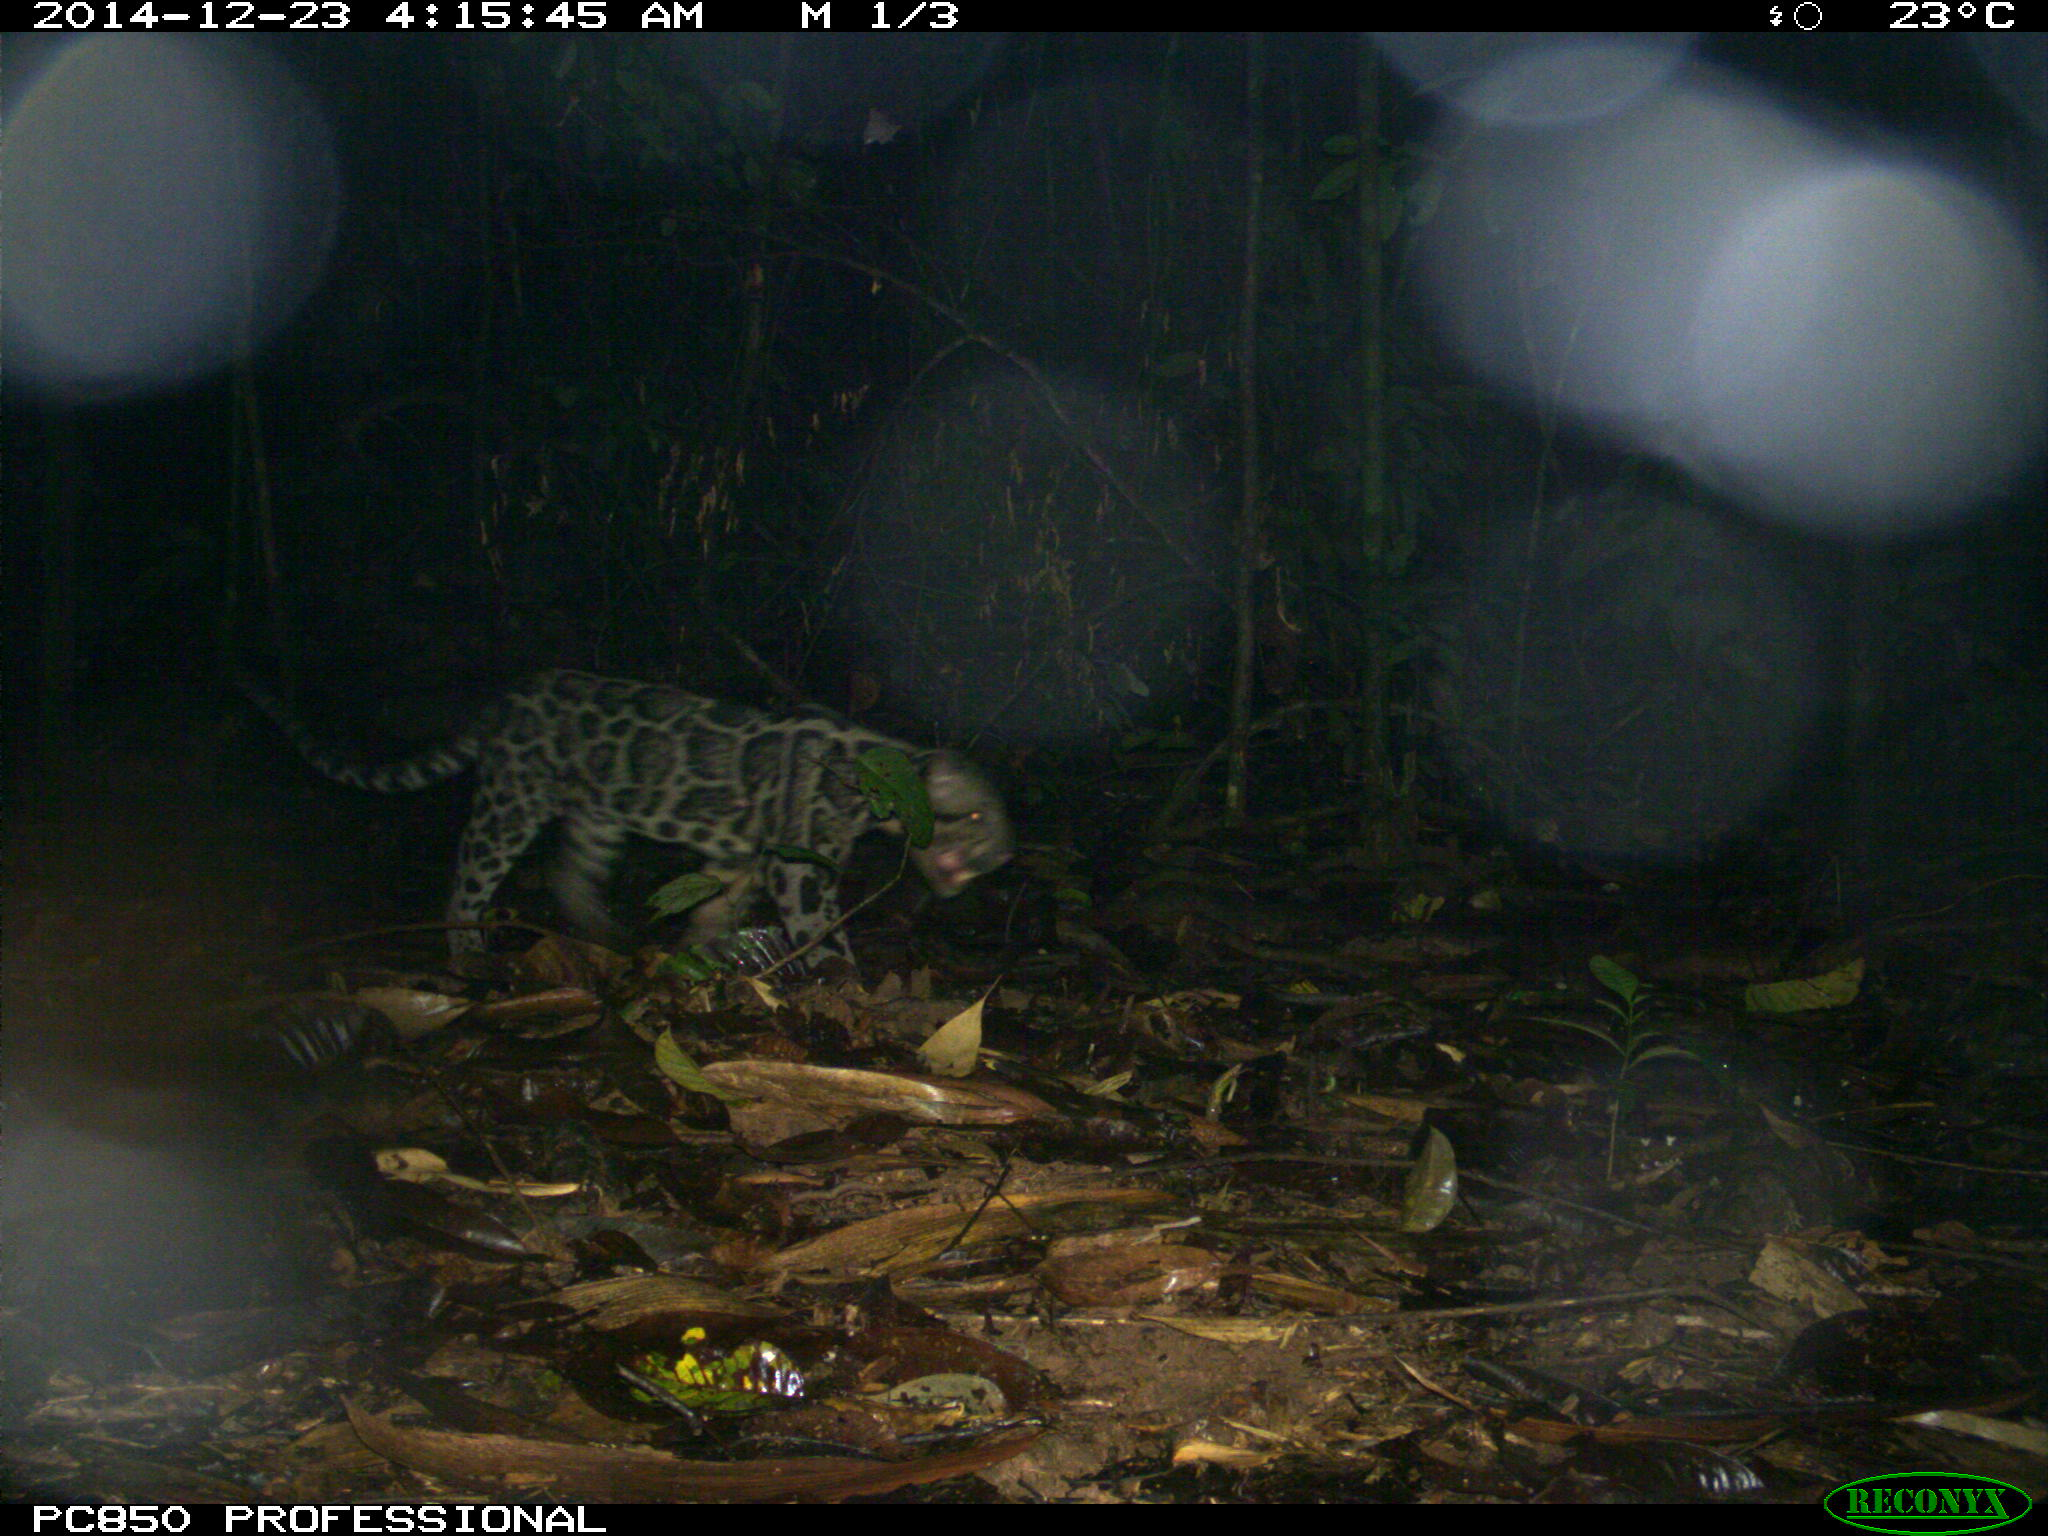
\includegraphics[width=\linewidth,height=\textheight,keepaspectratio]{images/example_DFR_2_male.JPG}
			\caption{DFR 2 male}
		\end{figure}
	\end{minipage}
	\hfill
	\begin{minipage}[c]{0.48\linewidth}
		\begin{figure}
			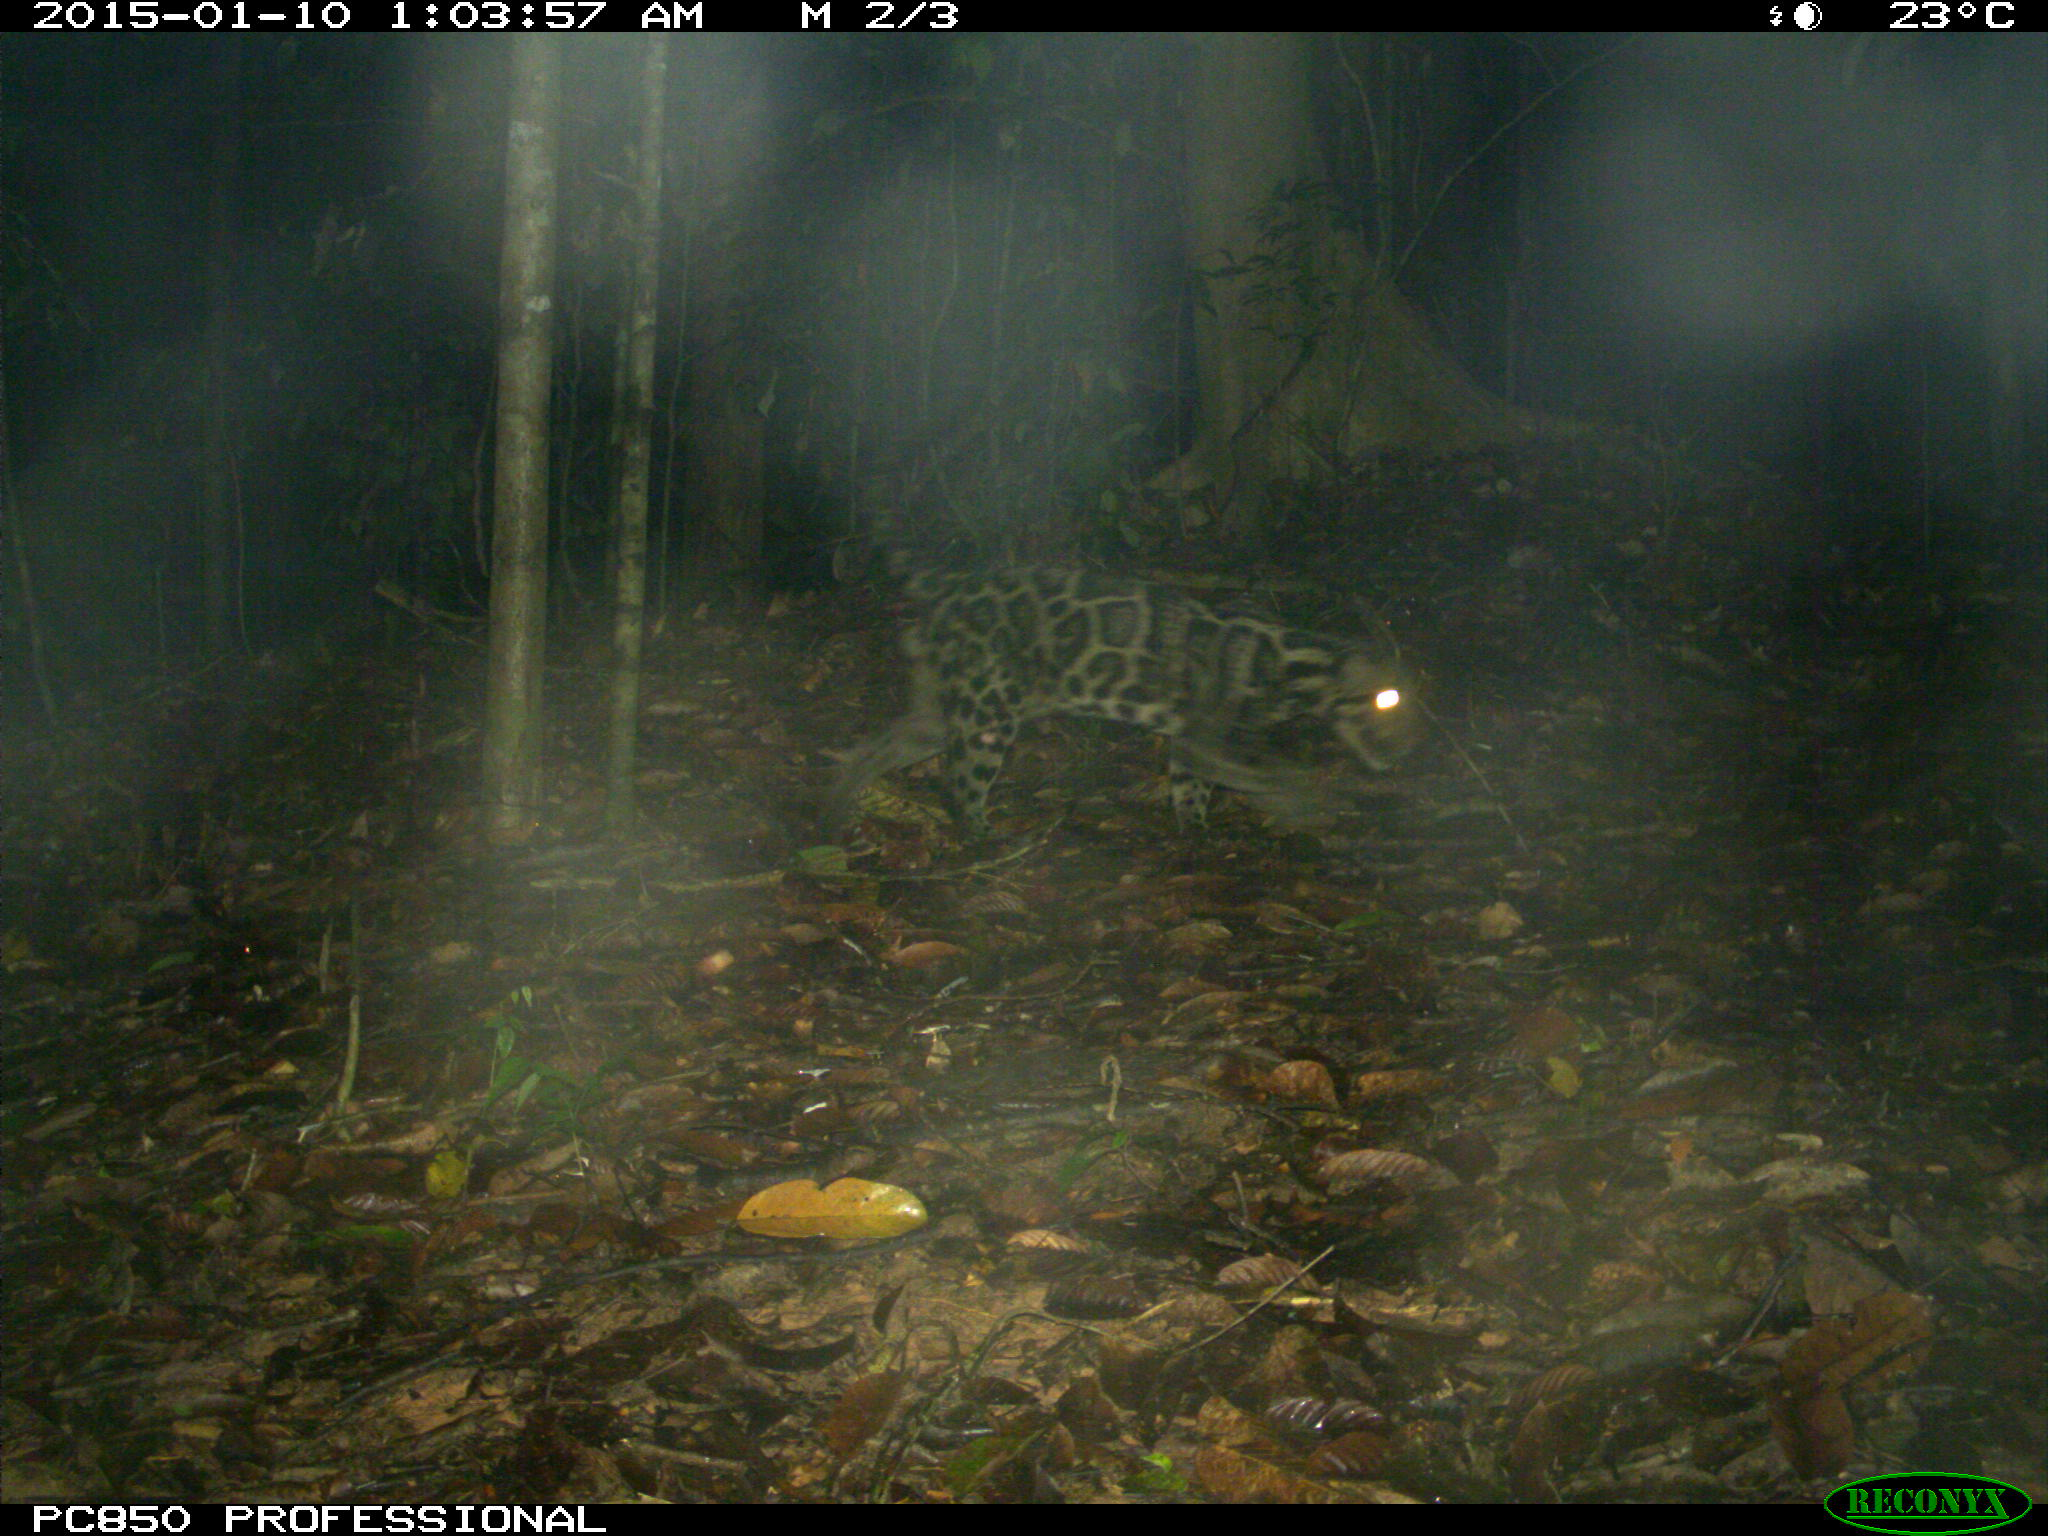
\includegraphics[width=\linewidth,height=.8\textheight,keepaspectratio]{images/example_DFR_5_male.JPG}
			\caption{DFR 5 male}
		\end{figure}
	\end{minipage}
\end{frame}

%-------------------------------------------------------
\subsection{Architecture}
%-------------------------------------------------------

\begin{frame}{Architecture}
	\begin{figure}
		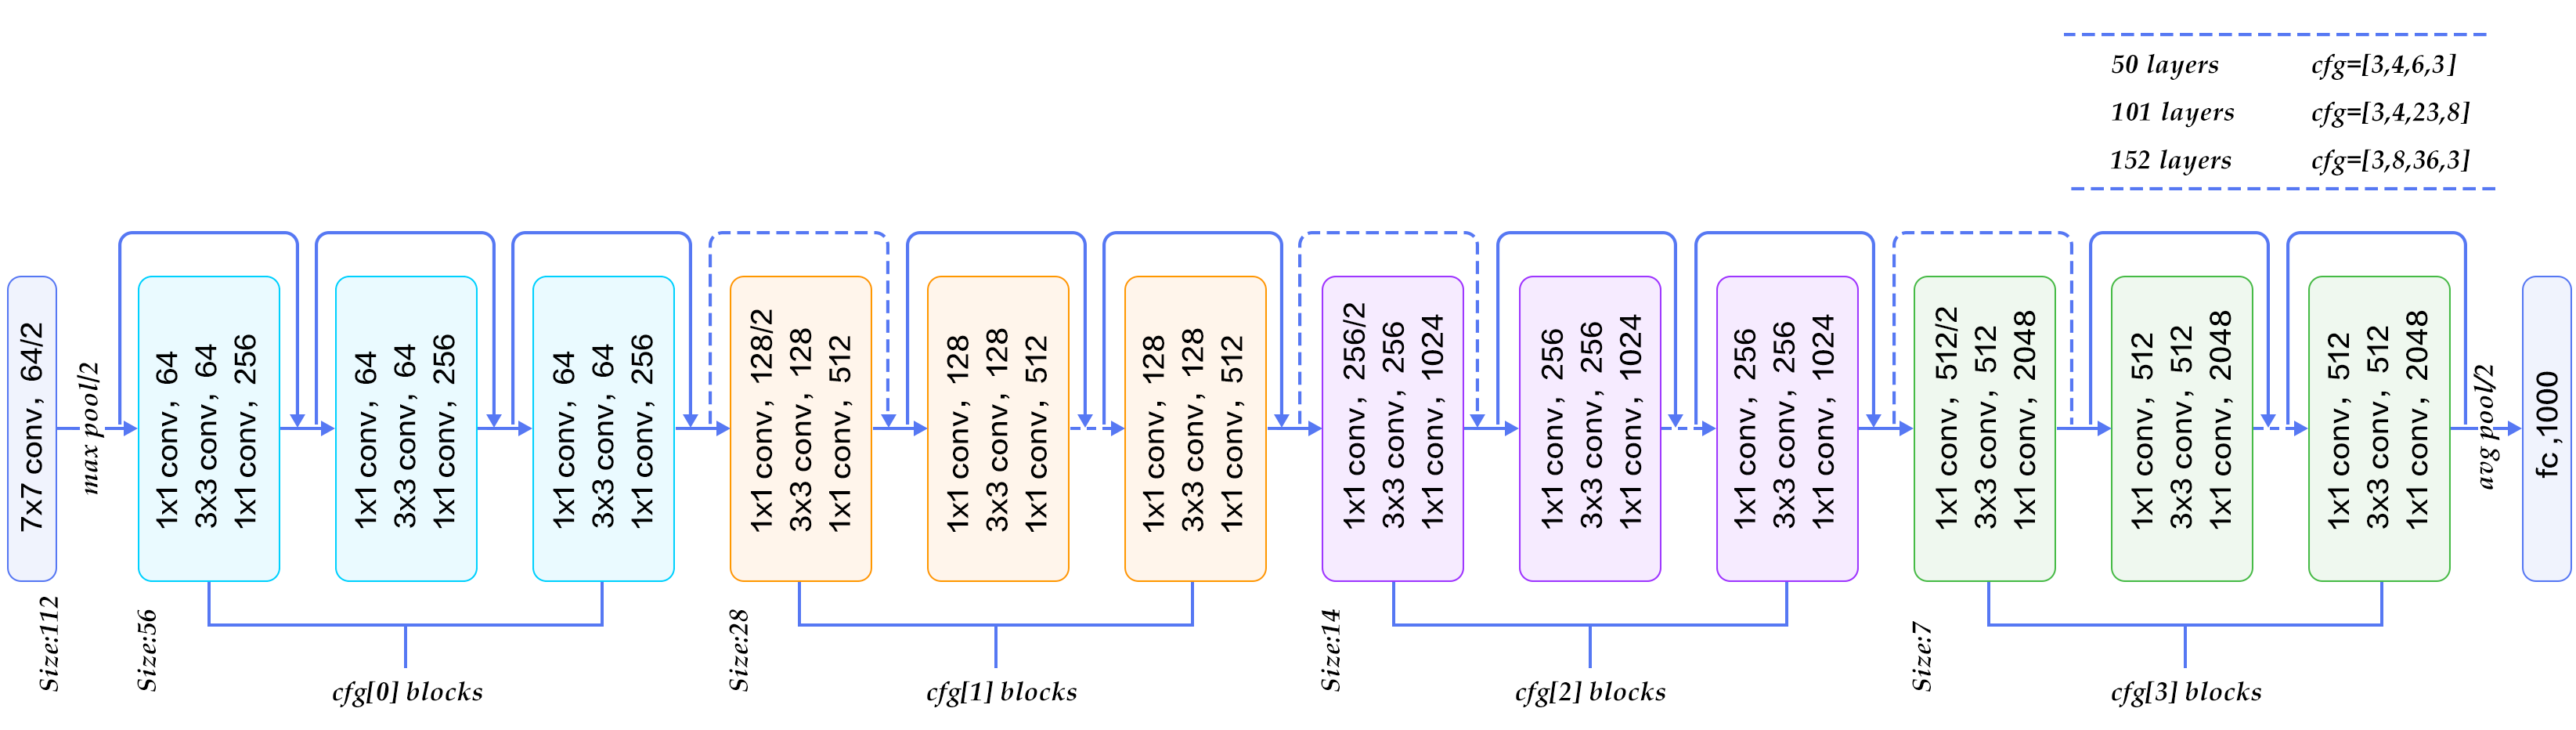
\includegraphics[width=\columnwidth]{images/resnet.png}
		\caption{ResNet Architecture\newline{} [\url{https://www.codeproject.com/Articles/1248963/Deep-Learning-using-Python-plus-Keras-Chapter-Re}]}
	\end{figure}

	\begin{itemize}
		\item ResNet-18, ResNet-34 from scratch
		\item ResNet-50 finetuning
	\end{itemize}
\end{frame}

%-------------------------------------------------------
\subsection{Results}
%-------------------------------------------------------

\begin{frame}{Scores}
	\centering
	\begin{minipage}[c]{0.58\linewidth}
		\begin{figure}
			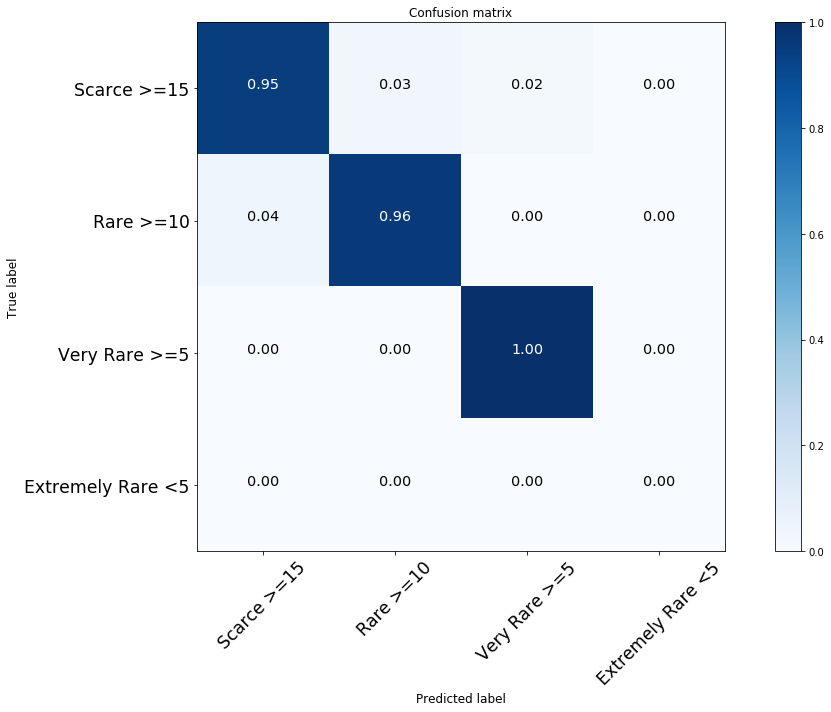
\includegraphics[width=\columnwidth]{images/conf_mat_leo_v2.png}
			\caption{Confusion matrix for finetuned Resnet-50}
		\end{figure}
	\end{minipage}
	\begin{minipage}[c]{0.38\linewidth}
		\textbf{Test set:}
		\begin{itemize}
			\item Accuracy: $0.91$
			\item Avg. Precision: $0.91$      
			\item Avg. Recall: $0.91$
			\item Avg. F1-Score: $0.90$
		\end{itemize}
	\end{minipage}
\end{frame}
%-------------------------------------------------------

\begin{frame}{Results}
	\centering
	\begin{figure}
		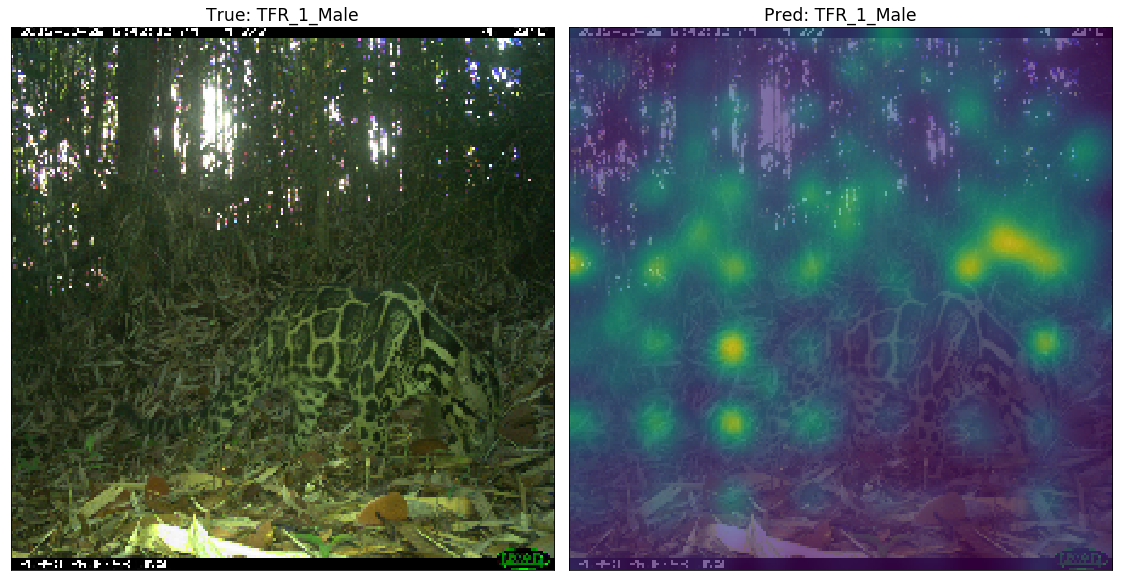
\includegraphics[width=\columnwidth]{images/result_leo_3.png}
		\caption{Network attention on background}
	\end{figure}
\end{frame}

%-------------------------------------------------------


\begin{frame}{Results}
	\centering
	\begin{figure}
		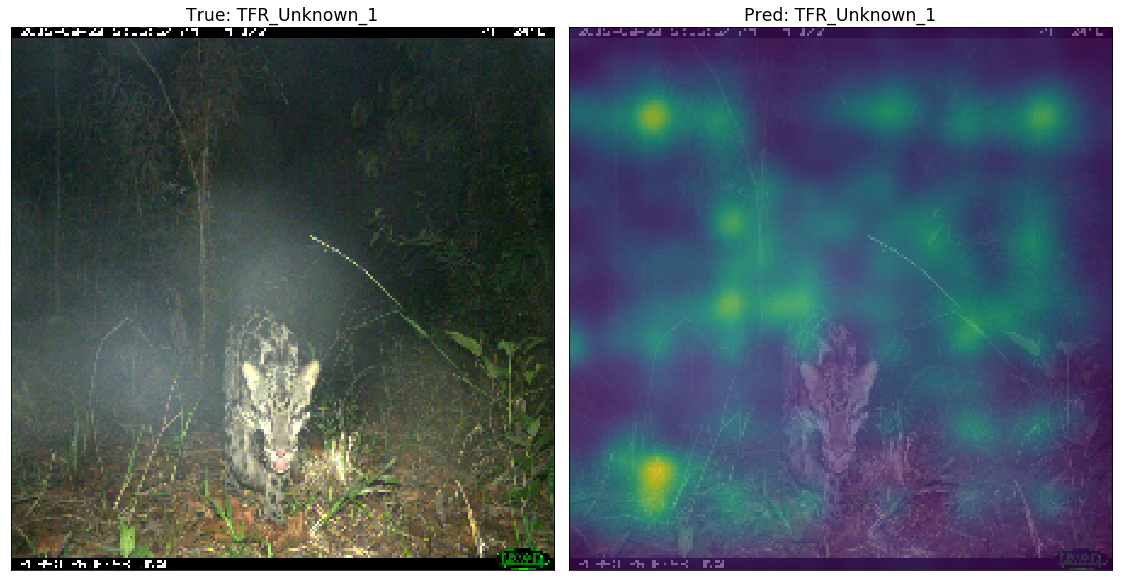
\includegraphics[width=\columnwidth]{images/result_leo_2.png}
		\caption{Network Attention on background}
	\end{figure}
\end{frame}

%-------------------------------------------------------

\begin{frame}{Training Process}
	\centering
	\begin{figure}
		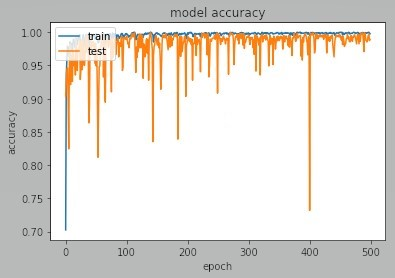
\includegraphics[width=.9\columnwidth,height=\textheight,keepaspectratio]{images/Pretrain_acc_ResNet50_cropped_heavy_augment_lr0_0001.jpg}
		\caption{Accuracy during Training}
	\end{figure}
\end{frame}

%-------------------------------------------------------

%\begin{frame}{Results}
%	\begin{figure}
%		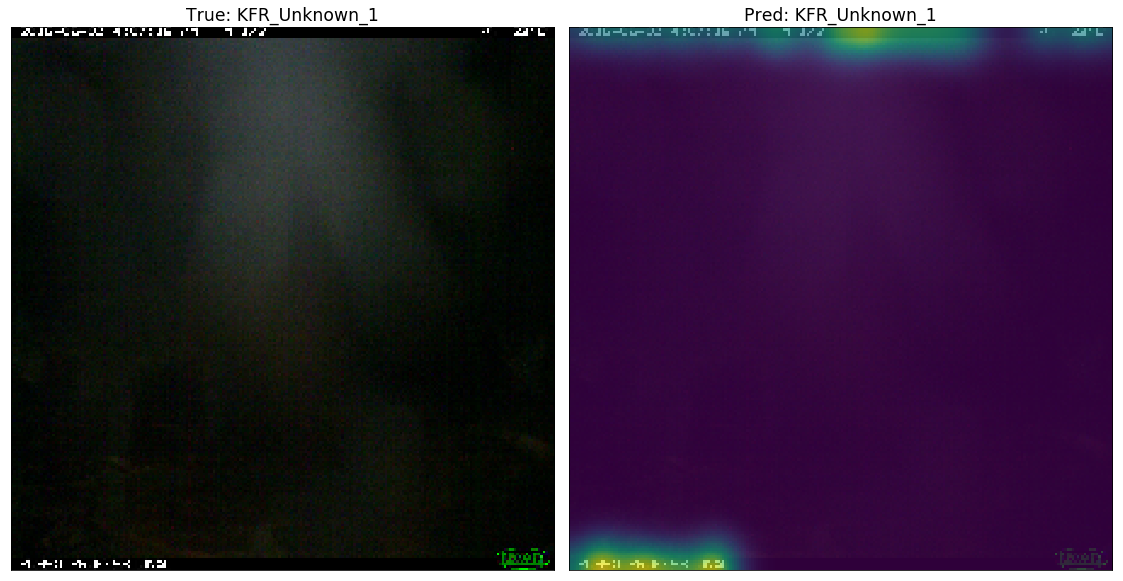
\includegraphics[width=\columnwidth]{images/Attention_Leo_Stamp.png}
%		\caption{Network Attention}
%	\end{figure}
%\end{frame}
%-------------------------------------------------------

\begin{frame}{Results}
	\begin{figure}
		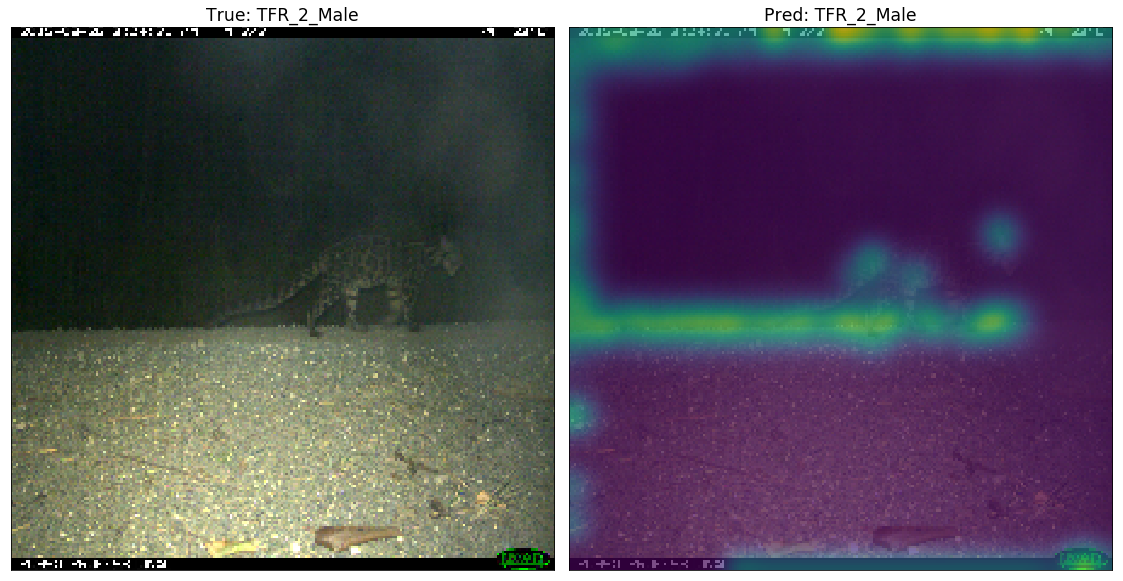
\includegraphics[width=\columnwidth]{images/Attention_Leo_Stamp2.png}
		\caption{Network attention on logo and time stamp}
	\end{figure}
\end{frame}

%-------------------------------------------------------
\subsection{Alternative Approach}
\begin{frame}{Using Bounding Boxes}
	\begin{figure}
		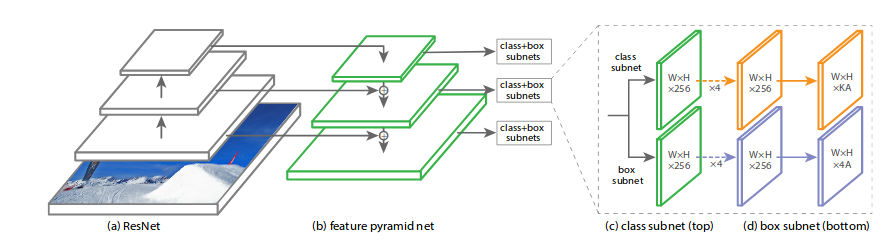
\includegraphics[width=\columnwidth]{images/retinanet.png}
		\caption{RetinaNet Architecture [\url{https://medium.com/@14prakash/the-intuition-behind-retinanet-eb636755607d}]}
	\end{figure}

	\begin{itemize}
		\item One stage detector with similar performance as Faster R-CNN
		\item Main improvement: Focal Loss
%		The novel focal loss focuses training on a sparse set of hard examples and prevents the vast number of easy negatives from overwhelming the detector during training.
%		\item losses semantic information an detect small objects RPN
%		\item used preferred backbone
%		\item extract after each pooling layer feature maps -- Feature pyramid network based on resnet
		\item Manual annotation of bounding boxes required
	\end{itemize}
\end{frame}

%-------------------------------------------------------

\begin{frame}{Scores}
	\centering
	\begin{minipage}[c]{0.58\linewidth}
		\begin{figure}
			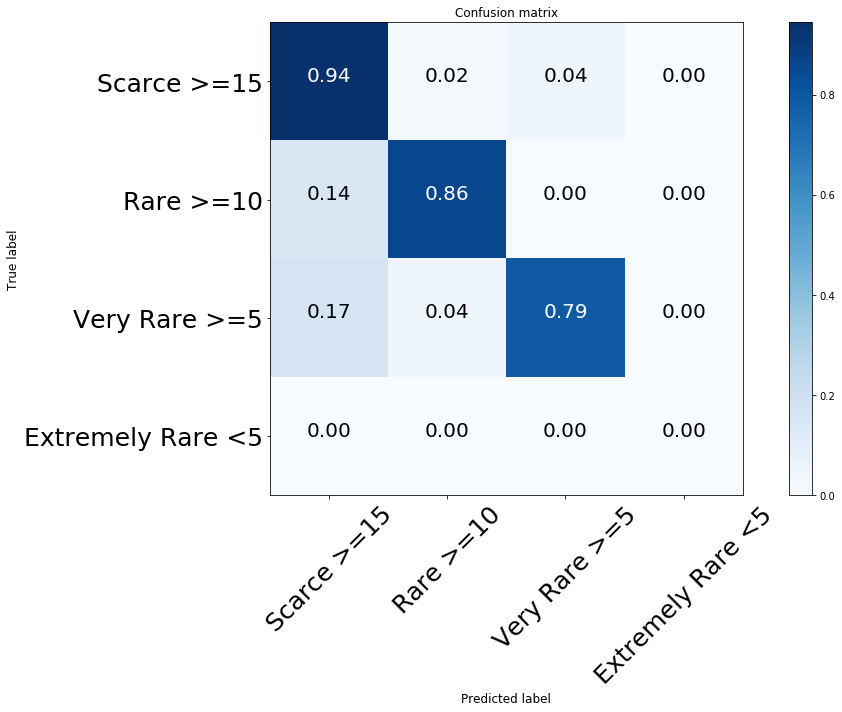
\includegraphics[width=\columnwidth]{images/conf_mat_leo_retina.png}
			\caption{Confusion matrix for finetuned RetinaNet with ResNet-50 backbone}
		\end{figure}
	\end{minipage}
	\begin{minipage}[c]{0.38\linewidth}
		\textbf{Test set:}
		\begin{itemize}
			\item Accuracy: 0.86
			\item Avg. Precision:  0.87
			\item Avg. Recall: 0.86
			\item Avg. F1-Score: 0.85
		\end{itemize}
	\end{minipage}
\end{frame}
%-------------------------------------------------------

\begin{frame}{Positive Examples}
	\centering
	\begin{figure}
		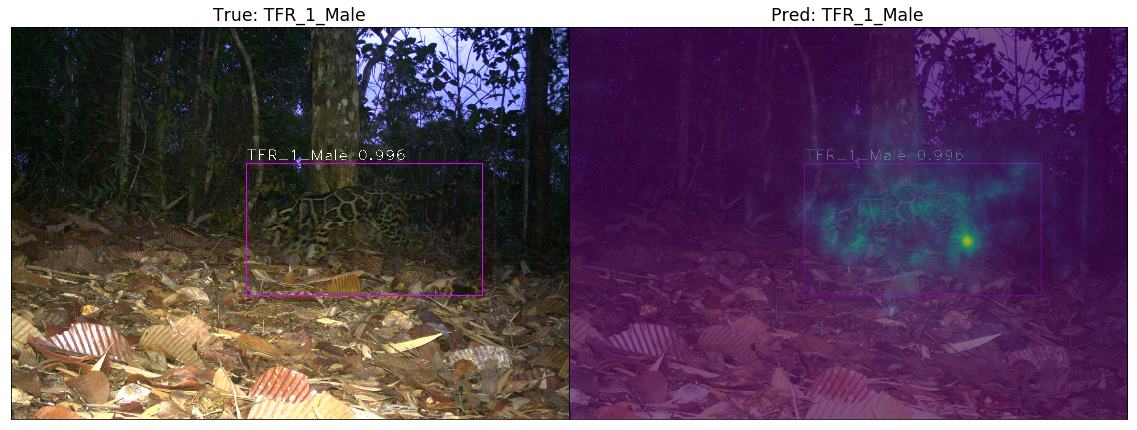
\includegraphics[width=\columnwidth]{images/RetinaNet_Attention_correct_good_quality2.png}
		\caption{RentinaNet attention on animal}
	\end{figure}
\end{frame}

%-------------------------------------------------------

\begin{frame}{Negative Examples}
	\centering
	\begin{figure}
		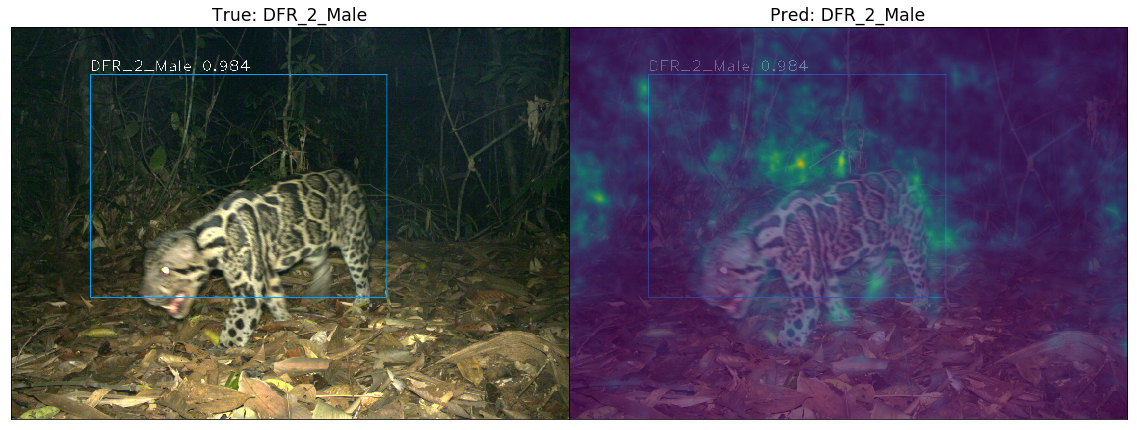
\includegraphics[width=\columnwidth]{images/RetinaNet_No_Attention_correct2.png}
		\caption{RentinaNet attention on background}
	\end{figure}
\end{frame}

%-------------------------------------------------------
\subsection{Finetuning for Individuals}
%-------------------------------------------------------

\begin{frame}{Finetuning for Individuals}
	\centering
	\begin{figure}
		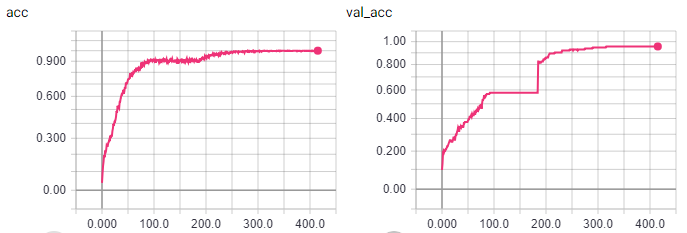
\includegraphics[width=.9\columnwidth,height=\textheight,keepaspectratio]{images/Acc_finetune_leo_both.png}
		\caption{Accuracy during training}
	\end{figure}
\end{frame}

%-------------------------------------------------------

\begin{frame}{Network Attention}
	\centering
	\begin{figure}
		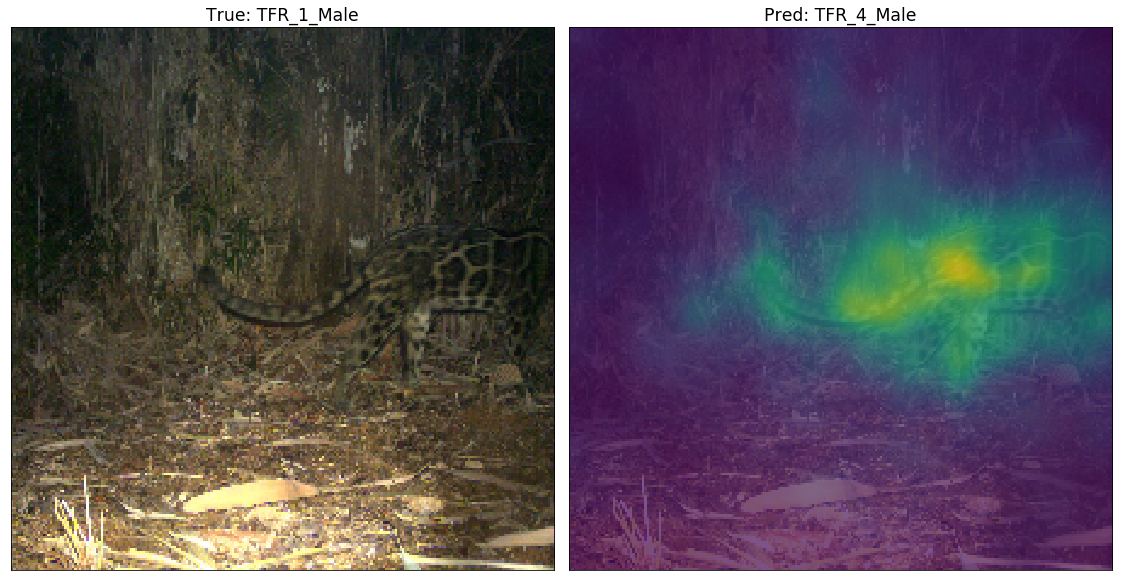
\includegraphics[width=\columnwidth]{images/finetune_Attention.png}
		\caption{Network attention after finetuning final dense layer}
	\end{figure}
\end{frame}

%-------------------------------------------------------

\begin{frame}{Network Attention}
	\centering
	\begin{figure}
		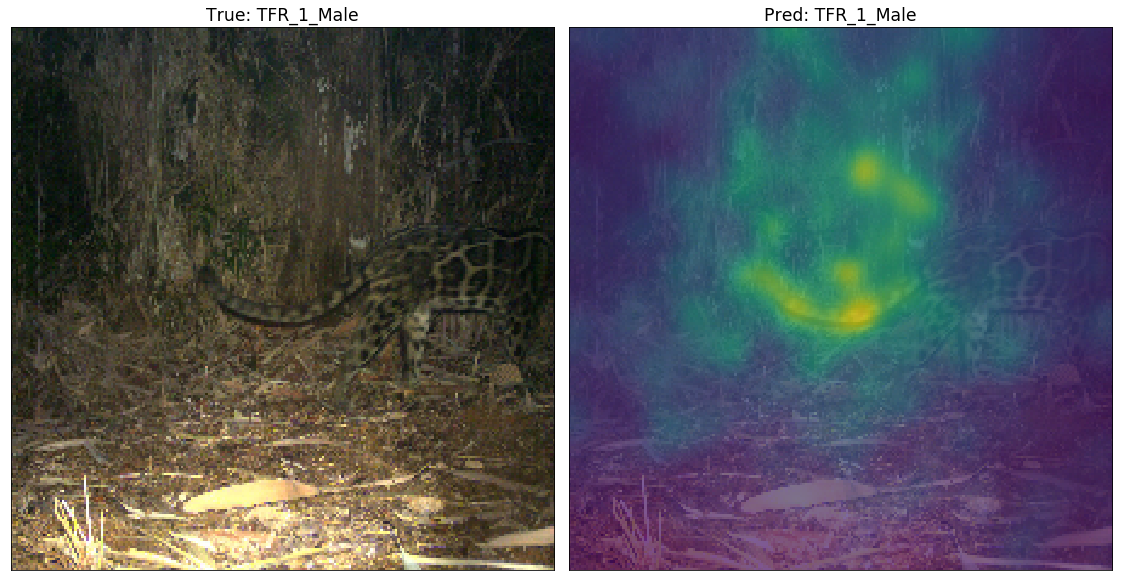
\includegraphics[width=\columnwidth]{images/finetune_Attention_later.png}
		\caption{Network attention after finetuning complete ResNet-50}
	\end{figure}
\end{frame}

%-------------------------------------------------------

{\1
\begin{frame}[plain,noframenumbering]
  \finalpage{Thank you for listening}
\end{frame}}

\end{document}